\documentclass[a4paper,12pt]{article}

\usepackage{tikz}\usetikzlibrary{calc}
\usepackage[utf8x]{inputenc}
\usepackage{ngerman}
\usepackage{amssymb}
\usepackage{graphicx}
\usepackage{pst-all}
\usepackage{Pakete/parallel} % erforderlich für die KVV-Einbindung
\usepackage{array}
\usepackage{longtable}
\usepackage{hyphenat}
\usepackage{rotating}
\usepackage{color}
\usepackage{multirow} % um in Tabellen etwas über mehrere Zeilen laufen zu lassen
\usepackage{Pakete/mylscape} % erforderlich für die Stundenpläne 
                              %   und KVV-Einbindung
\usepackage{amsmath}
\usepackage{hhline} %für doppellinien
\usepackage{multirow}
\usepackage{ulem}
\usepackage{eurosym} % Euro-Zeichen
%\usepackage{colortbl}

%\documentstyle[german,epsfig,12pt]{article}
\sloppy
%%%%%%%%%%%%%%%%%%
%% Seitenlayout %%
%%%%%%%%%%%%%%%%%%
\oddsidemargin0pt
\topmargin-1cm
\headheight0cm
\headsep0cm
\topskip1ex
\textheight24.5cm
\footskip1cm
\textwidth17cm
%%%%%%%%%%%%%%%%%%
%% Absatzlayout %%
%%%%%%%%%%%%%%%%%%
\setlength{\parindent}{0pt}
\setlength{\parskip}{5pt plus 2pt minus 1pt}
%%%%%%%%%%%%%%%%%%
%% Neue Befehle %%
%%%%%%%%%%%%%%%%%%
\newcommand{\strich}{\rule{11.85cm}{.4pt}\\}
\newcommand{\bfr}{\begin{flushright}}
\newcommand{\efr}{\end{flushright}}
\newcommand{\bc}{\begin{center}}
\newcommand{\ec}{\end{center}}
\newcommand{\be}{\begin{enumerate}}
\newcommand{\ee}{\end{enumerate}}
\newcommand{\bt}{\begin{tabular}}
\newcommand{\et}{\end{tabular}}
\newcommand{\bd}{\begin{description}}
\newcommand{\ed}{\end{description}}

%%%%%%%%%%%%%%
% Neue Fonts %
%%%%%%%%%%%%%%
\newfont{\cminch}{cminch scaled 1000}





















%%% Local Variables: 
%%% mode: latex
%%% TeX-master: "esi"
%%% End: 

\definecolor{grau}{gray}{0.8}
\definecolor{Pflicht}{gray}{0.5}
\definecolor{Basis}{gray}{0.6}
\definecolor{Aufbau}{gray}{0.7}
\definecolor{Wahl}{gray}{0.8}
\definecolor{Sonstiges}{gray}{0.9}

\def\colnr#1#2#3{\node at (#1*2.25cm,#2*1.5cm) {$#3$};}
\def\modul#1#2#3{\draw (#1*2.25cm,#2*1.5cm) node[minimum height=1.5cm,minimum width=2.25cm,draw] {\begin{minipage}{1.5cm}\begin{center}#3\end{center}\end{minipage}};}
\def\doublemodul#1#2#3{\draw (#1*2.25cm+1.125cm,#2*1.5cm) node[minimum height=1.5cm,minimum width=4.5cm,draw] {\begin{minipage}{3cm}\begin{center}#3\end{center}\end{minipage}};}
\def\twoofonemodul#1#2#3#4{\draw (#1*2.25cm+1.125cm,#2*1.5cm) node[minimum height=1.5cm,minimum width=4.5cm,draw] {\begin{minipage}{1.5cm}\begin{center}#3\end{center}\end{minipage}{\small oder}\begin{minipage}{1.5cm}\begin{center}#4\end{center}\end{minipage}};\draw (#1*2.25cm+1.125cm,#2*1.5cm+0.75cm) -- (#1*2.25cm+1.125cm,#2*1.5cm+0.25cm);\draw (#1*2.25cm+1.125cm,#2*1.5cm-0.25cm) -- (#1*2.25cm+1.125cm,#2*1.5cm-0.75cm);}
\def\eckmodul#1#2#3#4#5{\draw (#1*2.25cm-1.125cm,#2*1.5cm+0.75cm) -- (#1*2.25cm+3.375cm,#2*1.5cm+0.75cm);
\draw (#1*2.25cm-1.125cm,#2*1.5cm+0.75cm) -- (#1*2.25cm-1.125cm,#2*1.5cm-3.75cm);
\draw (#1*2.25cm-1.125cm,#2*1.5cm-3.75cm) -- (#1*2.25cm+1.125cm,#2*1.5cm-3.75cm);
\draw (#1*2.25cm+1.125cm,#2*1.5cm-3.75cm) -- (#1*2.25cm+1.125cm,#2*1.5cm-0.75cm);
\draw (#1*2.25cm+1.125cm,#2*1.5cm-0.75cm) -- (#1*2.25cm+3.375cm,#2*1.5cm-0.75cm);
\draw (#1*2.25cm+3.375cm,#2*1.5cm-0.75cm) -- (#1*2.25cm+3.375cm,#2*1.5cm+0.75cm);
\node at (#1*2.25cm+1.125cm,#2*1.5cm) {\begin{minipage}{3cm}\begin{center}#3\end{center}\end{minipage}};
\node at (#1*2.25cm,#2*1.5cm-0.75cm) {\small oder};
\node at (#1*2.25cm,#2*1.5cm-1.5cm) {\begin{minipage}{3cm}\begin{center}#4\end{center}\end{minipage}};
\node at (#1*2.25cm,#2*1.5cm-2.25cm) {\small oder};
\node at (#1*2.25cm,#2*1.5cm-3cm) {\begin{minipage}{3cm}\begin{center}#5\end{center}\end{minipage}};}

%ueberschriften (erforderlich für die KVV-Einbindungen)
\newcommand{\ueberschrift}[1]{\bf\huge{#1}}
\newcommand{\unterschrift}[1]{\rm\Large{#1}}

\setlength{\parindent}{0pt}
\setlength{\parskip}{5pt plus 2pt minus 1pt}

\setcounter{tocdepth}{2}

%In der Online-Version des ESIs sollten keine Copyright-geschützten Comics
%stehen, die in der gedruckten Version teilweise vorkommen. 
\newboolean{online}
\setboolean{online}{false} %gedruckte Version
%\setboolean{online}{true} %online-Version

%Verwendung im Code:
%\ifthenelse{\boolean{online}}
%{ hier steht, was in der online Version stehen soll
%}
%{ hier steht, was in der offline Version stehen soll
%}

%%%%%%%%%%%%%%%%%%%%%%%%%%%%%%%%%%%%%%%%%%%%%%%%%%%%%%%%%%%%%%%%%%%%%%%%
\begin{document}

%
% In dieser Datei bitte alle unten stehende Daten angeben.
% Die anderen tex-Files (z.B.: Einladung fuer die Erstsemester,
% ESI, ...) greifen darauf zurueck und nehmen die Ersetzungen
% selbststaendig vor.
%

% Jahreszahl
\newcommand{\Jahreszahl}{2016}

% Semester
\newcommand{\Semesterjahreszahl}{2016/2017}


% Wann findet die Erstsemestereinfuehrung statt?
\newcommand{\ESEWochentagEins}{Donnerstag}
\newcommand{\ESETagEins}{13}
\newcommand{\ESEWochentagZwei}{Freitag}
\newcommand{\ESETagZwei}{14}
\newcommand{\ESEMonat}{Oktober}

% Wann ist das ROMCE?
\newcommand{\ROMCEAnfang}{13}
\newcommand{\ROMCEEnde}{15}
\newcommand{\ROMCEMonat}{November}
         % Zum automatischen Einfügen der aktuellen Daten

\large
\thispagestyle{empty}
\begin{center}
{\Huge \bf
Informationsheft für Erstsemester
}
\\\rule{0cm}{1.5cm}
{\Large Wintersemester \Semesterjahreszahl}\\
\vspace{2cm}
{\huge Für die einen ist es ein gleichseitiges Dreieck mit
  Winkelhalbierenden und Inkreis.}

\begin{center}
\includegraphics[width=0.8\linewidth, clip]
{afs/.stud.mathe/fsmath/gemeinsame_Bilder/ESI/ESI_Logo}
\end{center}

\vspace*{-1cm}

{\huge Für die anderen ist es die kleinste projektive Ebene der Welt.}
\vspace*{\fill}
{\Large \ \\ Eine Serviceleistung der} \\[1ex]%\rule{0cm}{1.5cm}
{\huge \bf Fachgruppe Mathematik}
\end{center}

%%%%%%%%%%%%%%%%%%%%%%%%%%%%%%%%%%%%%
%%% Stand: 23. 09. 2014
%%%%%%%%%%%%%%%%%%%%%%%%%%%%%%%%%%%%%

\newpage
\vspace*{15cm}
{\small
\section*{Impressum} 
\begin{tabular}{@{}ll@{}} 
Herausgeber: & Fachgruppe Mathematik der Universität Stuttgart \\
 & Pfaffenwaldring 57\\
 & 70569 Stuttgart\\
 & Tel. (07 11) 685-653 41\\
 & E-Mail: fachgruppe@mathematik.uni-stuttgart.de\\
 & im Internet {\tt http://www.stud.mathematik.uni-stuttgart.de/Fachgruppe/}\\
V. i. S. d. P.:    & Anne Bernhardt\\
Redaktion und Layout: &Philipp Beck, Laura Sagarita, Tillmann Kleiner, Anja Herden, Andre Zieher\\
Titelbild: & Jörg Hörner, Jim Magiera \\
Druck: & Fachbereich Mathematik \\
Auflage: & 103 \\
Erscheinungsdatum: & 10. Oktober 2016 \\ \\
\multicolumn{2}{@{}l@{}}{\normalsize \it Alle Angaben in diesem Heft sind ohne
 Gewähr!}
\end{tabular}}

\newpage
\section*{Vorwort}
Hallo!

Willkommen an der Universität Stuttgart
und willkommen im Kreis der Mathe\-matikstudenten.
Bald geht dein Mathematikstudium los,
und wahrscheinlich hast du wenig Ahnung, 
wie dieses so ablaufen soll, welche Vorlesungen du
hören musst und und und\dots

Damit du dein Studium nicht ganz so hilf\-los beginnen musst,
geben wir für dich dieses Informationsheft heraus.
Hier steht das Wichtigste drin,
was du über dein Bachelorstudium als Mathematikstudent
oder Lehramtsstudent mit dem Fach Mathematik wissen solltest.
(Die hier enthaltenen Informationen haben wir
den jeweiligen Studienplänen und
Prüfungsordnungen nach bestem Wissen und Gewissen entnommen.
Die offiziellen Informationsquellen haben wir stets mit angegeben.
Das entbindet dich aber natürlich nicht,
dich auch selber zu informieren.
Insbesondere sind alle Angaben hier ohne Gewähr.)

%% Beachte bitte auch, dass wir am
%% {\bf \ESETagEins. und \ESETagZwei.~Oktober} eine
%% {\bf Erstsemestereinführung} veranstalten,
%% während der wir dir die wichtigsten Informationen
%% über dein Studium geben werden und du
%% uns noch alle offenen Fragen stellen kannst.

Wenn du Fragen hast oder in lockerer Atmosphäre
ein bisschen über das Studium plaudern willst,
schau doch einfach bei uns im Fachgruppenzimmer vorbei
- du bist immer herzlich willkommen!

\begin{flushright}{ \it Deine Fachgruppe Mathematik}
\end{flushright}
\vspace*{\fill}
{\small P.S.:\\
1.) Alle Personenbezeichnungen werden in diesem Heft
in männlicher Form verwendet,
beziehen sich aber selbstverständlich
auf alle Personen unabhängig vom Geschlecht.\\[2pt]
%2.) Die Lehramtsstudenten nach GymPO
%(\glqq altes\glqq\ modularisiertes Lehramt)
%bekommen von uns die Version des ESI des WS2014/15.
%Denn im GymPO hat sich von 2014 auf heute nichts geändert.\\[2pt]
2.) Am Dienstag Abend findet übrigens beinahe regelmäßig
unser Spieleabend statt.
Auch der ist ein Besuch wert.}

\includepdf[pages=-]{plakat_16_17.pdf} 
%%%%%%%%%%%%%%%%%%%%%%%%%%%%%%%%%%%%%%%%%%
%% Stand: 03. Oktober 2016
%%%%%%%%%%%%%%%%%%%%%%%%%%%%%%%%%%%%%%%%%%

\newpage
{\tableofcontents}
\vspace*{3cm}

\newpage
\begin{center}
\includegraphics[width=\textwidth]
{/afs/.stud.mathe/fsmath/gemeinsame_Bilder/Comics/titelbg1}
\end{center}

\vspace{-3cm}

\section{Studieren an einer Universität}

In diesem Heft wollen wir dir erklären,
was du alles machen musst,
um deinen Bachelor of Science
bzw.\ dein Bachelor of Arts
für's Lehramt zu erreichen.
Dabei erläutern wir dir den Ablauf
deines zukünftigen Studienalltags,
der sich unter Anderem in Vorlesungen,
Übungsgruppen, Seminare, Prüfungen am Semesterende
und so weiter gliedert...

\subsection{Das Bachelorstudium}

Das Studium für den Bachelor of Science in Mathematik
ist auf sechs Semester ausgelegt und
kann grob in zwei Abschnitte unterteilt werden.
Während der ersten drei Semester
sollst du die elementaren Grundlagen
der Mathematik erlernen,
die für fast alle darauf aufbauenden Spezialisierungen
oder gar Anwendungen unverzichtbar sind.
Auch lernst du die \glqq mathematische Art,
Wissenschaft zu betreiben
und Probleme zu lösen\grqq.

Darunter fällt die formale Beschreibung
mathematischer Sachverhalte, Beweisführung etc.,
an denen sich das Vorgehen in {\it allen}
Teilgebieten der Mathematik orientiert.
In diesem Abschnitt sind die meisten Studieninhalte fest vorgegeben.
Du kannst dir aber zum Beispiel dein Nebenfach
frei nach belieben aussuchen.
Im Gegensatz dazu kannst du dann im zweiten Teil
das meiste frei aus einem Pool an Vertiefungen auswählen.
Wo du dann schließlich deine Bachelorarbeit schreibst,
hängt von deiner Entscheidung und dem Angebot ab.

Ein vollständiges Lehramtsstudium
teilt sich auf in ein Bachelorstudium
nach dessen erfolgreichen Abschluss
du den Titel \glqq Bachelor of Arts\grqq\ erhältst,
und einen Masterstudiengang,
den du mit dem Titel \glqq Master of Education\grqq\ abschl\-ießt.
Du kannst die mathematischen Grundlagenvorlesungen
bereits in den ersten drei Semestern erwerben
und die Priorität zunächst auf die Mathematik legen
oder deren Erwerb auf vier Semester strecken
und dafür dem Zweitfach etwas mehr Priorität geben.
Die erste Möglichkeit hat den Vorteil,
dass dein Studium besser mit dem Verlauf
des Studiums deiner Kollegen im Bachelor of Science harmoniert.
Als Lehramtsstudent besteht dein Studium
auch noch aus dem Zweitfach und Veranstaltungen zur Pädagogik.

Nach bestandenem Bachelorstudium erhältst du den Titel
\glqq Bachelor of Science\grqq\ bzw.\ 
\glqq Bachelor of Arts\grqq\  zusammen mit dem
\glqq Diploma Supplement\grqq, einem langen Begleitheft,
in dem ausführlich drinsteht,
was du während deines Studiums geleistet hast.

Hast du deinen \glqq Bachelor of Science\grqq\ 
in Mathematik erworben, besteht die Möglichkeit,
ein viersemestriges Masterstudium in Mathematik anzuschließen,
das allerdings mit Zulassungsvoraussetzungen verbunden ist.

Hast du als Lehramtsstudent
deinen \glqq Bachelor of Arts\grqq\ erworben,
geht es normalerweise mit dem \glqq Master of Education\grqq\ weiter.
Zusätzlich oder alternativ kannst du auch ein Ergänzungsstudium beginnen,
um zu deinem \glqq Bachelor of Arts\grqq\ 
den \glqq Bachelor of Science\grqq\  in Mathematik zu erwerben.

% Für Lehrämtler geht der erste Studienabschnitt bis zum vierten Semester,
% dann folgt das Praxissemester an einer Schule.
% Danach folgen nochmal fünf Semester an der Uni.
% Im ersten Studienabschnitt ist ziemlich genau festgelegt,
% welche Vorlesungen du besuchen und welche Prüfungen du ablegen musst.
% Hast du alle notwendigen Leistungen erbracht,
% erhältst du deine sogenannte \glqq Zwischenprüfung\grqq.
% Dabei handelt es sich um keine echte Extra-Prüfung,
% sondern nur um eine Ansammlung deiner bisher erbrachten Studienleistungen.

%Da du als Lehrämtler gleich zwei Fächer studieren musst, kann es vorkommen, dass eine der beiden Zwischenprüfungen (eine in Mathematik und eine in dem anderen Fach) erst nach dem fünften Semester abgeschlossen wird. Maximal hast du sechs Semester Zeit, deine Zwischenprüfung abzulegen; ansonsten verlierst du bundesweit den Prüfungsanspruch und wirst exmatrikuliert.

\subsection{Module}
Das Studium ist in sogenannte Module eingeteilt.
Ein Modul kann eine oder mehrere Veranstaltungen wie
z.B.\ eine Vorlesung, ein Seminar oder ein Computerpraktikum beinhalten.
Die Module werden in der Regel benotet.
Zusätzlich bekommt man für jedes bestandene Modul,
unabhängig von der Note,
die ihm zugeordneten \glqq Leistungspunkte\grqq (LP).
Damit wird der geschätzte Arbeitsaufwand
zum Bewältigen des Moduls gewürdigt.
Ein Leistungspunkt entspricht ungefähr 30 Stunden.
Ein Modul mit 9 LP bedeutet also 270 Stunden Arbeit.
Dies schließt z.B.\ den Besuch der Vorlesung, Nacharbeitung,
Prüfungsvorbereitung etc.\ mit ein.

Zum Erwerb des Bachelorgrades benötigt man zusammen mindestens 180 LP.
Für die Lehramtsstudenten fallen während des Bachelorstudiums
78 LP bis 84 LP für den Mathematikteil an,
je nachdem ob du in Mathematik oder in deinem Zweitfach
deine Bachelorarbeit schreiben möchtest.
18 LP sind für die Bildungswissenschaften reserviert,
der Rest ist für das Zweitfach.

Im Masterstudiumsabschnitt fallen nochmals 120 LP an.
Für die Lehramtsstudenten sind davon 77 LP für die Fächer,
sowie 27 LP und 16 LP für Bildungswissenschaft bzw.\ Schulpraxis.

\subsection{Vorlesungen}

Die Vorlesungen sind die zentralen Lehrveranstaltungen an Universitäten.
Dort stellt euch der Dozent mathematische Lehrsätze und
Rechenmethoden vor, führt Beweise aus, und eure Aufgabe ist es,
dazu Aufschriebe anzufertigen und so gut wie möglich
die Gedankengänge zu verfolgen.
Im Grundstudium sitzt ihr dabei zu Hundertschaften in einem Hörsaal.
%% Wenn Ihr später speziellere Vorlesung hört,
%% kommt es vor, daß ihr zu fünft in einer Vorlesung hockt.

In 90 Minuten kann eine ganze Menge Stoff vorgetragen werden
und zwar meist deutlich mehr, als ein durchschnittlicher Student
in dieser Zeit vollständig verdauen kann.
Falls du in einer Vorlesung nicht alles auf Anhieb verstehst,
hin und wiedermal den Faden verlierst,
ist das noch kein Weltuntergang;
vielen anderen Hörern geht es genauso.
Die Vorlesungen müsst ihr daher regelmäßig,
je nach Geschmack für euch allein
oder in kleinen Gruppen, nacharbeiten.

Die Arbeit alleine hat den Vorteil,
daß jeder in seinem Tempo lernen kann
und man weniger abgelenkt wird
($\Rightarrow$ \glqq Lernflow, Effizienz\grqq).
Die Gruppenarbeit hat den Vorteil,
daß man auch mit den Fragen der Kollegen konfrontiert wird,
und Dinge so erläutern muss, dass einen die Kollegen auch verstehen.
So kann man nebenbei seinen Lernerfolg überprüfen
($\Rightarrow$ \glqq Interaktion, Qualitätskontrolle\grqq).
Jeder muss da seine optimale Mischung finden.

Häufig tauchen während einer Vorlesung Fragen auf:
der eine Beweisschritt ist unklar,
die durchgeführte Rechnung ist nicht nachvollziehbar,
oder die Rechnung ist zu Ende, aber du siehst das Ergebnis noch nicht.
In diesen Fällen ist es erlaubt den Dozenten zu fragen.
Meist freuen sich die Dozenten über Nachfragen
und ermutigen daher auch die Hörerschaft dazu.
Solche Chancen lohnt es sich zu nutzen,
denn ein bisschen Interaktion macht die Vorlesung
auch stets etwas lebendiger!
Vereinzelt wird dabei auch ein harmloser Schreibfehler aufgedeckt,
der die Hörerschaft durcheinander gebracht hat.

\vspace{2cm}

\begin{center}
\includegraphics[width=12cm]
{/afs/.stud.mathe/fsmath/gemeinsame_Bilder/Comics/labyrinth_puzzle}
\end{center}

\subsection{Übungen und Scheine}

Zu den Vorlesungen werden Übungen angeboten.
Diese dienen zur Vertiefung der Vorlesungsinhalte,
zur Übung der erlernten Rechen-
oder Beweisführungsmethoden, sowie dem Scheinerwerb.
Um an der Prüfung des zugehörigen Moduls teilnehmen zu können,
musst du nämlich in der Regel einen Schein erwerben,
indem du erfolgreich an einer Übungsgruppe teilnimmst.
Zu dieser muss man sich stets anmelden.

Die zum Scheinerwerb notwendigen Leistungen werden stets
{\it Scheinbedingungen} oder {\it Scheinkriterien} genannt.
Um diese zu erfüllen musst du in der Regel einen gewissen Prozentsatz
von Aufgaben erfolgreich bearbeitet haben,
die wöchentlich vom Dozenten oder
einem Assistenten veröffentlicht werden.

Den Nachweiß erbringst du zum Beispiel durch:\\[6pt]
- {\bf Schriftliche Abgaben}\\[2pt]
- {\bf Bearbeitung von Präsenzaufgaben, Kurztests}\\[2pt]
- {\bf Vorrechnen an der Tafel}\\[2pt]
- {\bf Aktive Mitarbeit in der Übungsgruppe}\\
\hspace*{0.5cm}(vor allem regelmäßige Teilnahme)\\[6pt]
Manchmal wird zusätzlich eine Scheinklausur geschrieben,
deren Bestehen notwendig für den Erhalt des Scheins ist.

{\it Die genauen Scheinbedingungen legt der jeweilige Dozent fest.
Welche Bedingungen für euch gelten,
und auch wie man sich für die Übungsgruppen anmeldet,
erfährst du in den ersten Vorlesungen des Semesters.}

Die Übungsgruppen werden je nach Dozent/Assistent unterschiedlich organisiert.
Die beiden häufigsten Arten sind:\\[6pt]
- {\bf Votierübungen}\\[2pt]
- {\bf Präsenzübungen}\\[6pt]
In einer {\it Votierübung} wird zu Beginn
stets ein Votierzettel verteilt,
auf dem die Teilnehmer der Übung ankreuzen (=\glqq votieren\grqq),
welche Aufgaben sie erfolgreich bearbeitet haben.
Der Übungsgruppenleiter, auch Tutor genannt,
wählt dann aus der Liste jemandem zum Vorrechnen aus,
der dann seinen Lösungweg an der Tafel präsentiert.
In der Regel sollte man 2-3 mal vorgerechnet haben
um einen Schein zu erhalten.

In der {\it Präsenzübung} könnt ihr euch wie ihr wollt
in Kleingruppen zusammen setzen und euch daran machen,
das Aufgabenblatt der Woche zu bearbeiten.
Dabei schlendert der Tutor durch den Raum,
schaut euch ein bisschen über die Schulter
und kann euch auch die ein oder andere Hilfestellung geben.

Während der Übungsgruppe habt ihr reichlich Gelegenheit
Fragen zu stellen, die euch der hilfsbereite
und kompetente Tutor gerne beantwortet,
oder die in der Gruppe diskutiert werden können.
Schriftliche Abgaben und Kurztests werden in der Regel
vom Tutor korrigiert und ihr erhaltet eure Abgaben
mit Bewertung eine Woche später wieder zurück.

Eine Übungsgruppe besteht in der Regel aus 15 bis 25 Studenten.
In den Übungsgruppen herrscht also meist eine lockerere Atmosphäre.
Man lernt sich untereinander schneller kennen
als in Vorlesungen und stellt eher mal eine Frage.
Daher können sie für ein erfolgreiches Studium enorm hilfreich sein.

Was kann man mit einem Schein anfangen?
Will man die Prüfung zu einem Modul ablegen,
ist der Schein meist die Zulassungsvoraussetzung zur Prüfung.
Aber selbst wenn nicht, empfehlen wir {\bf dringend},
zu jeder besuchten Vorlesung auch den zugehörigen Schein zu erwerben.
Hast du einmal einen Schein in einer Übung erworben,
aber möchtest die zugehörige Prüfung erst später schreiben,
z.B.\ ein Jahr später, so kannst du ihn dann anerkennen lassen
und die Prüfung mitschreiben.

\subsection{Proseminare und Hauptseminare}
\label{Proseminar}
Jeder muss im Laufe seines Studiums Seminare besuchen.
Die Studenten des Bachelor of Science
machen ein Proseminar und ein Hauptseminar. 
Lehramtsstudenten im Bachelor of Arts
machen ein Proseminar.

Ein Seminar läuft folgendermaßen ab:
Jeder Teilnehmer bekommt einige Seiten
aus einem Buch oder ein Thema mit Literaturliste zugeteilt.
Diese muss er dann gründlich durch- und zu einem Vortrag ausarbeiten.
Jede Woche im Semester steht dann einer dieser Teilnehmer
vorne an der Tafel und hält seinen Vortrag.
Der betreuende Dozent hört sich diese Vorträge
an und stellt zwischendurch ein paar Fragen
zum Verständnis des Stoffes.
Natürlich sollte der Vortragende diese Fragen
dann auch möglichst souverän beantworten können.
Es kann außerdem eine schriftliche Ausarbeitung
des Themas verlangt werden. 
Wenn der Dozent mit dem Vortrag
und der Ausarbeitung zufrieden war und wenn man nicht
allzu oft im Semester gefehlt hat,
besteht man das Modul, bekommt die Leistungspunkte gutgeschrieben
und eine Note (es gibt keine extra Prüfung).

Pro- und Hauptseminare unterscheiden sich nur im Schwierigkeitsgrad. 
In der Regel findet am vorletzten Mittwoch
in der Vorlesungszeit (Aushänge beachten!)  eine Seminarplatzvergabe statt,
auf der die Seminare und fachdidaktischen Übungen des folgenden
Semesters vorgestellt und die Plätze vergeben werden.

\subsection{Computermathematik}

Die Studenten des Bachelor of Science
müssen im ersten Semester die Veranstaltung
\glqq Mathematik am Computer\grqq~besuchen.
Hier erlernt man Basistechniken (Unix, \LaTeX, ...)
und eine Einführung in Mathematiksoftware (Maple, Mathematica, Matlab, ...).
Zudem wird es (als Block am Ende des Semesters)
einen \glqq Programmierkurs\grqq\ geben.
Die Teilnahme an diesem ist eine Zulassungsvoraussetzung
für die Teilnahme an der Modulprüfung Mathematik am Computer Prüfung.

Zusammen mit der Vorlesung \glqq Numerische Lineare Algebra\grqq
~im zweiten Semester bilden diese drei Veranstaltungen das Modul
\glqq Grundlagen der Computermathematik\grqq.

Im fünften Semester gibt für die Studenten
des Bachelor of Science das \glqq Computerpraktikum Mathematik\grqq.
Im Verlauf dieses Praktikums müsst ihr in Dreiergruppen
drei Aufgabenstellungen mit Hilfe
von C++, MatLab oder anderen Programmen bearbeiten.

Für die Lehramtsstudenten im Bachelor of Arts
gibt es das Modul angewandte Mathematik.
Dieses besteht aus den Veranstaltung \glqq Wahrscheinlichkeitstheorie\grqq,
\glqq Numerische Lineare Algebra\grqq\ und dem \glqq Programmierkurs\grqq.

\subsection{Prüfungen}

Die meisten Module schließt ihr am Ende
des Semesters durch die Teilnahme
an der Modulprüfung ab (die ihr hoffentlich besteht).
Die Prüfung findet schriftlich oder mündlich statt
und dauert in der Regel 120 Minuten bzw.\ 30 Minuten.
Sie ist bestanden, wenn man die Note 4,0 oder besser hat.
Falls man durchgefallen ist -- d.h. man hat die Note 5,0 --
muss man die Prüfung wiederholen.

\subsubsection{Zulassungsvoraussetzungen}\label{sssec:zu}

Um zur Modulprüfung zugelassen zu werden,
brauchst du in der Regel den Übungsschein
der entsprechenden Übungsgruppe.
Steht in der Modulbeschreibung des Modulhandbuchs (siehe \ref{ssec:fp} unten)
{\it Zulassungsvoraussetzung XY},
so must du den Übungsschein des Moduls {\it XY}
ebenfalls erworben haben,
um zur Prüfung zu gelassen zu werden.
So brauchst du z.B.\ um die \glqq Wahrscheinlichkeitstheorie\grqq-Prüfung
mitschreiben zu dürfen den Übungsschein
zur Wahrscheinlichkeitstheorie,
aber auch die zu Analysis~I+II.

\subsubsection{Prüfungsanmeldung}\label{sssec:pa}

Zu Prüfungen müsst ihr euch stets rechtzeitig anmelden.
Die Anmeldung zu einer Prüfung erfolgt
für die Studenten des Bachelor of Science
über das LSF
und für die Lehramtsstudenten im Bachelor of Arts
über das C@MPUS-Managementsystem.

Eure Anmeldung müsst ihr innerhalb
des {\it Prüfungsanmeldezeitraums} erledigen.
Dieser ist geht im ersten Semester
vom {\bf 18.~November bis zum 10.~Dezember}.

{\bf LSF:}
\begin{enumerate}
\item
Besuche die Seite {\small\verb|lsf.uni-stuttgart.de|}.
\item
Logge dich mit deiner Kennung matXXXXX und deinem Passwort ein.
\item
Klicke auf \glqq Prüfungsanmeldung und -rücktritt\grqq,\\
in der Menuleiste auf der linken Seite.
\end{enumerate}
In der Liste, die rechts erscheint
kannst du nun das Modul auswählen,
zu dessen Prüfung du dich anmelden willst.\\
{\it Die Anmeldung zur Prüfung über das LSF ist verbindlich.
Innerhalb einer Frist vor der Prüfung
kann man sich ohne Angabe von Gründen abmelden.
Beachte dazu auch die Hinweise im LSF-Portal.}

{\bf C@MPUS:}\\
Man muss sich Einloggen und
so etwas ähnliches wie im LSF machen.
Weitere Details werden noch bekannt gegeben,
da die Autoren bisher niemanden kennen, der sich über C@mpus
zu einer Klausur angemeldet hat.

\subsubsection{Orientierungsprüfung}\label{sssec:or}

Für die Studenten des Bachelor of Science
zählen die Prüfungen zu zwei der Module Analysis I \& II
und LAAG I \& II als Orientierungsprüfung,
für Lehrämtler im Bachelor of Arts die Prüfung im Modul LAAG I.

Orientierungsprüfung heißt: die genannten Module
musst du bis spätestens zum Beginn der Vorlesungszeit
des vierten Semesters erfolgreich bestanden haben.
Keine Panik, das schaffst du schon,
viele vor dir haben ihre Prüfungen
schließlich auch geschafft.

{\it Vergleiche mit der Prüfungsordnung Bachelor of Science Mathematik} §6~(1) in:\\
{\small
\verb|http://www.uni-stuttgart.de/zv/bekanntmachungen/bekanntm_27_2012.pdf|}\\
Beziehungsweise in der {\it Prüfungsordnung Bachelor of Arts Lehramt} §6~(1) in:\\
{\small
\verb|http://www.uni-stuttgart.de/zv/bekanntmachungen/bekanntm_55_2015.pdf|}\\
Sowie 8.~§1 auf S.\ 16 im {\it besonderen Teil} der {\it PO für BA Lehramt} in:\\
{\small
\verb|http://www.uni-stuttgart.de/zv/bekanntmachungen/bekanntm_56_2015.pdf|}

\subsubsection{Wiederholung von Prüfungen}\label{sssec:wi}

{\bf Im Bachelor of Science Mathematik:}\\
Bestandene Prüfungen können grundsätzlich nicht wiederholt werden.
Jede nichtbestandene Prüfung darf einmal wiederholt werden.
Als Termin für deine Wiederholungsprüfung
musst du allerspätestens den übernächsten Prüfungstermin wahrnehmen.
Häufig wird eine Wiederholungsklausur angeboten.

Außerdem darf man im Laufe seines Studiums
in maximal vier Fällen eine nichtbestandene Prüfung
ein zweites Mal wiederholen (gilt nicht für die Module,
die zur Orientierungsprüfung gehören).
Der letzte Rettungsanker:
Fällt man durch die schriftliche Wiederholungsprüfung
eines Orientierungsprüfungsfachs
oder durch die zweite schriftliche Wiederholungsprüfung
einer anderen Vorlesung, so erfolgt zeitnah eine 20-30 Minuten
dauernde mündliche Fortsetzungsprüfung (hier entscheidet sich die Note
nur noch zwischen 4,0 oder 5,0).
Wer das auch nicht packt, verliert seinen Prüfungsanspruch
für den Bachelor in Mathematik
in ganz Deutschland und wird exmatrikuliert.

{\it Vergleiche auch mit der Prüfungsordnung BSc Mathematik} §18:\\
{\small
\verb|http://www.uni-stuttgart.de/zv/bekanntmachungen/bekanntm_27_2012.pdf|}

{\bf Im Bachelor of Arts Lehramt Mathematik:}\\
Jede nichtbestandene Prüfung darf einmal wiederholt werden,
danach gibt es eine mündliche Nachprüfung.
Desweiteren kann man drei Prüfungen aus dem Mathematikteil
und zwei aus dem Teil Bildungswissenschaften,
die keine Orientierungsprüfungen sind,
jeweils zweimal wiederholen.
Die Wiederholungsprüfung muss {\it innerhalb
von zwei Semestern} abgelegt werden.
Fällt man durch eine Orientierungsprüfung
oder das zweite mal durch eine andere Prüfung,
muss man {\it zeitnah} zur einer mündlichen Prüfung antreten,
bei der man nur noch Aussicht auf die Noten 4,0 oder 5,0 hat.
Besteht man auch diese nicht,
so verliert man seinen Prüfungsanspruch.

{\it Vergleiche auch mit der Prüfungsordung Lehramt Mathematik} §20:\\
{\small
\verb|http://www.uni-stuttgart.de/zv/bekanntmachungen/bekanntm_55_2015.pdf|}

Wie ihr seht, ist der Prüfungsmodus sehr human.
Es bedarf viel, um endgültig durchzufallen.
Trotzdem solltest du es nicht darauf anlegen.
Zum einen gehen viele eurer Prüfungsergebnisse
auch in eure Endnote mit ein,
zum anderen stehen die Ergebnisse
in eurem \glqq Diploma Supplement\grqq.
Wir raten auch davon ab, Prüfungen aufzuschieben.
Die Arbeitslast wird dadurch immer größer.

\subsection{Fristen und Studienplanung}\label{ssec:fp}

Hier nochmal eine kurze Zusammenfassung
aller prüfungsrechtlich relevanten Fristen
in deinem Studium.\\[6pt]
- {\bf Orientierungsprüfung:}\\
\hspace{1cm}{\it Bis spätestens zum Beginn des 4.~Semesters} (siehe \ref{sssec:or})\\[3pt]
- {\bf Abschluss deines Bachelors:} (d.h.\ {\it das Bestehen aller Module})\\
\hspace{1cm}{\it Bis spätestens zum Ende des 10.~Semesters}\\[3pt]
- {\bf Prüfungswiederholung im Bachelor of Science Mathematik:}\\
\hspace{1cm}{\it Spätestens beim übernächsten möglichen Termin}
(siehe \ref{sssec:wi})\\[3pt]
- {\bf Prüfungswiederholung im Bachelor of Arts Lehramt:}\\
\hspace{1cm}{\it Spätestens innerhalb von zwei Semestern}
(siehe \ref{sssec:wi})\\[3pt]
- {\bf Prüfungsmeldezeitraum:} (siehe \ref{sssec:pa})\\[6pt]
Solange du dich an diese Fristen hältst,
kannst du dein Studium sonst theoretisch völlig frei gestalten.
Musst/Möchtest du zum Beispiel dein Studienleben
durch zusätzliche zeitintensive Hobbies bereichern
(Segelfliegen, Musik, Marathonlaufen, Familie, Geld verdienen, etc.),
so spricht nichts dagegen dies tun.

\newpage
Der Studienplan liefert dir eine Orientierung,
in welcher Reihenfolge du die Vorlesungen besuchen solltest.
Wirklich relevant für dein Planung ist,
welche Module Voraussetzung für andere Module sind,
zu denen du eine Prüfung schreiben willst
und welche Module obligatorisch,
d.h.\ ein bisschen wichtiger sind.

Solltest du eine oder mehrere Prüfungen nicht bestehen
(selbstverständlich wirst du alles daran legen,
dass es nicht soweit kommt)
musst du deine Studienplanung eventuell anpassen.

Beziehst du das BAföG, so ist zu beachten,
dass dieses in der Regel nur bis zum Ende
des 6.~Semesters gezahlt wird,
d.h.\ solange du in der sogenannten
\glqq Regelstudienzeit\grqq\ bleibst.

Vor Beginn eines jeden Semesters kannst du dir schon überlegen,
welche Vorlesungen du besuchen möchtest.
Dazu gibt es einige Informationsmöglichkeiten:

1. {\bf Die Mathematik-Homepage {\verb|www.mathematik.uni-stuttgart.de|}:}
Über\\ 
$ \sim ${\verb|/fachbereich/studium/vorlesungen/index.html|}\\
kommst du schnell an alle wichtigen Informationen zu den Vorlesungen.
Mit \glqq Studium\grqq\ $\Rightarrow$ \glqq Lehrveranstaltungen\grqq 
kannst du dich auch zu diesen Infos durchklicken.
Falls du weiter in die Zukunft blicken willst, kannst du auch\\
$ \sim ${\verb|/fachbereich/studium/vorlesungen/vorlesungsplanung/index.html|}\\
besuchen.


2. {\bf Das LSF-Portal:}\\
{\verb|lsf.uni-stuttgart.de|}\\
Links in der Menüleiste auf \glqq VVZ + Semester\grqq\ klicken,
der Rest erklärt sich von selbst.
Dort kannst du auch unter \glqq Modulhandbuch
und Prüfungsordnung\grqq\ nachschlagen.
Dort findet man unter Anderem
auch die empfohlenen inhaltlichen Voraussetzungen
sowie die prüfungsrechtlich bindenden
Zulassungsvoraussetzungen zu den Prüfungen der Module.

3. {\bf Das C@mpus-Portal:}\\
{\verb|campus.uni-stuttgart.de|}\\
Um hier die Vorlesungen einzusehen, gehst du auf deine Visitenkarte.
Dein Weg setzt sich mit einem Klick auf Studienstatus fort und mit
eine weiteren Klick auf deinen Studiengang bist du am Ziel.

\newpage
\subsection{Prüfungsausschussvorsitzende und andere wichtige Personen}

Bei allen Fragen zur Prüfungsordnung
kann dir der Vorsitzende des Prüfungsausschusses weiterhelfen.
Das ist für den Bachelor Mathematik:\\
Herr Apl.~Prof.~Dr.~Christian Hesse\\
Zimmer: 8.317\\
Telefon: (0711) 685 - 65343\\
E-Mail: Christian.Hesse@mathematik.uni-stuttgart.de

Die Studiendekanin für den  Bachelor ist
Frau Prof. Dr. Uta Freiberg\\
Zimmer: 8.550\\
Telefon (0711) 685 - 66647\\
E-Mail:  uta.freiberg@mathematik.uni-stuttgart.de

\label{LAzust}
Für das Lehramt gibt es einen eigenen Prüfungsausschussvorsitzenden:\\
Herr Prof. Dr. Jürgen Pöschel
Zimmer:  8.560\\
Telefon: (0711) 685 - 65523\\
E-Mail: Juergen.Poeschel@mathematik.uni-stuttgart.de

Der Studiendekan fürs Lehramt ist
Herr Prof. TeknD Timo Weidl\\
Zimmer: 8.347\\
Telefon (0711) 685 - 65534\\
E-Mail: Timo.Weidl@mathematik.uni-stuttgart.de

Falls du auf Lehramt studierst
und nebenbei mit nur wenig Aufwand
zusätzlich einen Bachelor machen möchtest,
dann wende dich an\\
Herr apl. Prof. Kimmerle\\
Zimmer: 7.344\\
Telefon: (0711) 685 - 65323\\
E-Mail: Wolfgang.Kimmerle@mathematik.uni-stuttgart.de

Bei Fragen oder Unklarheiten zum Bachelor
oder Lehramt kann man sich
bei der Studiengangsmanagerin melden:\\
Frau Dr. Friederike Stoll
Zimmer:  7.553 \\
Telefon: (0711) 685 - 65515 \\
E-Mail: stoll@mathematik.uni-stuttgart.de

{\it Auch zu finden auf der Mathematik-Homepage unter \glqq Fachbereich\grqq\ 
$\Rightarrow$ \glqq Ansprechpartner\grqq\ etc...}
\\
\subsection{Tipps und Tricks für das Mathematikstudium}
Das Wichtigste wollen wir dir nicht vorenthalten,
das Mathestudium wird kein Spaziergang.
Aber wir wollen dich auch nicht beunruhigen,
sondern dich vor Fallen warnen, in die viele von uns getappt sind.
Wir raten dir:
\begin{itemize}
\item
Nicht abschrecken lassen, wenn es nicht auf Anhieb klappt.
Achte mal darauf, dass es den meisten so geht.

\item
Aus diesem Grund gemeinsam arbeiten.
Im Gegensatz zu dem Klischee ist es wichtig untereinander zu kommunizieren.

\item
Frag so oft und so viel wie du kannst.
Habe keine Angst, dass deine Frage zu einfach ist.
Aus der höheren Perspektive ist sie das meistens.

\item
Du solltest Zeit für Übungsaufgaben einplanen.
Wichtig ist, dass die meiste Zeit für Aufgaben und nicht für die
Vorlesung drauf geht.
\end{itemize}
Leider gibt es kein allgemeines Kochrezept um am Ball zu bleiben,
dies musst du für dich selbst rausfinden.
Den Meisten hilft es jedoch erfahrungsgemäß
\begin{itemize}
\item
die Vorlesung zu besuchen und nachzuarbeiten.
\item
Übungsblätter nicht einfach abzuschreiben.
\end{itemize}
Das mit dem Abschreiben ist fundamental wichtig,
sonst wirst du höchstwahrscheinlich bei den ersten Scheinklausuren
ziemlich auf die Schnauze fliegen.
Aber vergiss auch nicht,
dass es seine Zeit braucht,
um sich an die Denkweise in der Mathematik zu gewöhnen.

Auch wichtig ist,
sich von dem Gesagten nicht abschrecken zu lassen und gelassen zu bleiben.
Wahrscheinlich begibst du dich in eine dir unbekannte Welt,
dass dies meistens nicht reibungslos abläuft sollte klar sein.

Wir wissen, dass wir uns wiederholen.
Aber es ist wichtig sich nicht unterzukriegen zu lassen,
dann wirst du eine Menge Spaß mit der Mathematik haben.
  
\newpage
\vspace*{4cm}
\ifthenelse{\boolean{online}}
{

}
{
\begin{center}
  \includegraphics[width=12cm]{/afs/.stud.mathe/fsmath/gemeinsame_Bilder/Comics/comic41}
\end{center}
}
\newpage

%%%%%%%%%%%%%%%%%%%%%%%%%%%%%%%%%%%%%%%%%%
%% Stand: 03. Oktober 2016
%%%%%%%%%%%%%%%%%%%%%%%%%%%%%%%%%%%%%%%%%%


\newpage
\section{Studienplan für den Bachelor of Science}

Die Module des Bachelorstudiengangs
teilen sich in drei Gruppen auf.
Es gibt Mathematikmodule, Nebenfachmodule (24 LP)
und Schlüsselqualifikationen (sog. \glqq Soft-skills\grqq, 18 LP).

\subsection{Mathematikmodule}
Zunächst einmal die Auflistung aller Mathematikmodule
im Laufe deines sechs-semestrigen Bachelorstudiums
(das Computerpraktikum zählt offiziell als Schlüsselqualifikation).
Die Semesterangaben im folgenden sind stets
nicht prüfungsrechtlich bindend.

%\vspace*{-0.5cm}

\begin{center}
\includegraphics[width=17cm]
{afs/.stud.mathe/fsmath/gemeinsame_Bilder/Friederike/Bachelor.pdf}
\end{center}

Der obige Plan gibt dir eine Orientierung darüber,
in welcher Reihenfolge du die Vorlesungen besuchen solltest.
Solltest du z.B.\ Analysis~I nicht beim ersten Versuch bestehen,
heißt das nicht, daß du erst ein Jahr aussetzen musst,
bevor mit Analysis~II anfangen kannst.
Du versucht einfach die wichtigsten Inhalte von Analysis~I
soweit nachzuholen, daß du in Analysis~II noch mitkommst.
Möglicherweiße bestehst du dann Analysis~II
und schreibst dann deine Wiederholungsprüfung
für Analysis~I einfach im 3.~Semester.
Diese Möglichkeit soll verhindern,
daß sich dein Studium nicht unnötig verzögert.

Beachte stets die Zulassungsvoraussetzungen
für spätere Module (siehe \ref{sssec:zu}).

\subsubsection{Der Grundlagenteil (typischerweise 1. - 3. Semester)}

Der Grundlagenteil besteht aus folgenden {\bf Pflichtmodulen}:\\[6pt]
- {\bf Analysis~I-III}\\[2pt]
- {\bf Lineare Algebra und Analytische Geometrie~I-II}  (LAAG I-II)\\[2pt]
- {\bf Grundlagen der Computermathematik}\\[6pt]
Das Modul \glqq Grundlagen der Computermathematik\grqq
~geht über zwei Semester und setzt sich aus der 1+1 Veranstaltung
\glqq Mathematik am Computer\grqq ~im ersten Semester,
einem \glqq Programmierkurs\grqq, der als Blockveranstaltung
in der vorlesungsfreien Zeit stattfindet,
und der 2+1 Lehrveranstaltung \glqq Numerische Lineare Algebra\grqq
~im zweiten Semester zusammen.

Außerdem besucht man im dritten Semester noch zwei {\bf Basismodule}.
Dazu wählt man zwei aus folgenden drei Modulen:\\[6pt]
- {\bf Topologie}\\[2pt]
- {\bf Numerische Mathematik~I}\\[2pt]
- {\bf Wahrscheinlichkeitstheorie}\\[6pt]
Die Module werden in der Regel
durch eine schriftliche Prüfung (120 min) abgeschlossen.
Für die drei Module werden Analysis~I+II
und LAAG~I+II als Voraussetzung empfohlen.
%braucht man für die ersten beiden Analysis- bzw.\ LAAG-Vorlesungen
%jeweils den dazugehörigen Übungsschein.
Für das Modul \glqq Grundlagen der Computermathematik\grqq
\ braucht ihr die Scheine des Programmierkurs
%und der Veranstaltung \glqq Mathematik am Computer\grqq
und die Prüfung in \glqq Numerische Lineare Algebra\grqq.

Zwei Prüfungen der Module \glqq Analysis I \& II\grq
~und \glqq LAAG I \& II\grqq~dienen zugleich
als sogenannte {\it Orientierungsprüfung}.
Sie müssen bis zum Beginn der Vorlesungszeit des vierten Fachsemester
erfolgreich bestanden sein.

{\bf Achtung:}
Viele Vorlesungen aus dem zweiten Studienabschnitt erfordern
bestimmte Basis- oder Aufbaumodule als Voraussetzung.
Ihr legt also bei der Wahl der Basismodule
schon eine thematische Ausrichtung eures weiteren Studiums fest.
Auf der anderen Seite kann euch niemand davon abhalten
zusätzliche Vorlesungen zur Ergänzung zu hören,
falls ihr zum Beispiel eure thematische Ausrichtung wechseln wollt.

\newpage
\subsubsection{Der Vertiefungsteil (typischerweise 4. - 6. Semester)}

Ihr müsst unter anderem
drei der folgenden fünf {\bf Aufbaumodule} absolvieren:\\[6pt]
- {\bf Algebra}\\[2pt]
- {\bf Geometrie}\\[2pt]
- {\bf Höhere Analysis}\\[2pt]
- {\bf Numerische Mathematik~II} (Voraussetzung: Numerische Mathematik~I)\\[2pt]
- {\bf Mathematische Statistik} (Voraussetzung: Wahrscheinlichkeitstheorie)\\[6pt]
Am Ende dieser Aufbaumodule findet jeweils eine Prüfung statt.
Wie diese genau abläuft, wird vom Dozenten zu Beginn festgelegt. 

Der Vertiefungsteil dient zudem der Spezialisierung.
Dazu besucht ihr\\
  - {\bf Vertiefungsmodule}\\
  - ein {\bf Computerpraktikum Mathematik} und\\
  - ein {\bf Mathematisches Seminar}.

Das \glqq Mathematische Seminar\grqq\ 
besteht aus einem Proseminar und einem Hauptseminar.
Das Proseminar wird meist im dritten oder vierten Semester besucht,
das Hauptseminar im fünften oder sechsten Semester.
Im Gegensatz zu den meisten Vorlesungen
werden Pro- und Hauptseminare jeweils
in den Sommer- {\it und} Wintersemestern angeboten.

Habt ihr euch durch das Bestehen von Modulen
genügend Leistungspunkte (90 LP) erarbeitet,
dürft ihr mit eurer Bachelorarbeit beginnen.
Hier sollt ihr weitgehend selbstständig
eine umfangreiche, aber klar abgesteckte
mathematische Aufgabenstellung schriftlich ausarbeiten.

\subsubsection{Endnote}

Eure Endnote in der Mathematik
setzt sich aus dem nach Leistungspunkten
und Studienabschnitt gewichteten (Analysis 1-3, LAAG 1-2,
Grundl. der Computermathematik, Computerpraktikum und Basismodule ~=~Faktor~1; \\
Aufbau-, Vertiefungsmodule und Seminar ~=~Faktor~2; Bachelorarbeit~=~Faktor~3)
Durchschnitt der Noten der einzelnen Mathematikmodule zusammen
und wird auf eine Stelle nach dem Komma gerundet.

%\begin{tabular}{lcrl}
%  Mathenote & = & $\frac{9}{231} \, \cdot$ & (Analysis I + Analysis II + Analysis III)\\[0.5ex]
%            & + & $\frac{9}{231} \, \cdot$ & (LAAG I + LAAG II + Basis I + Basis II)\\[0.5ex]
%            & + & $\frac{6}{231} \, \cdot$ & (Grundlagen der Computermathematik)\\[0.5ex]
%            & + & $\frac{18}{231}\, \cdot$ & (Aufbau I + Aufbau II + Aufbau III + Aufbau IV)\\[0.5ex]
%            & + & $\frac{18}{231}\, \cdot$ & Vertiefung\\[0.5ex]
%            & + & $\frac{12}{231}\, \cdot$ & (Ergänzung + Computerpraktikum + Seminar)\\[0.5ex]
%            & + & $\frac{36}{231}\, \cdot$ & Bachelorarbeit\\
%\end{tabular}

Eure {\bf Gesamtnote} setzt sich zu $13/15$ aus der Mathenote
und zu $2/15$ aus der Nebenfachnote zusammen.
Bei Wahl von speziellen Vertiefungsmodulen ist die Gesamtzahl
der Leistungspunkte nicht 180, sondern 183 oder 186.

\begin{center}
\includegraphics[width=11cm]
{afs/.stud.mathe/fsmath/gemeinsame_Bilder/Comics/comic2}
\end{center}

\subsection{Nebenfachmodule}

Zusätzlich zu den Mathematikmodulen
musst du eines der nachfolgenden Nebenfächer besuchen.
Die hier angegebenen Semester der jeweiligen Veranstaltungen
sind nur Empfehlungen, keine Pflicht. 
Soweit es möglich war, haben wir angegeben,
welchen Umfang (Vorlesung + Übung) die jeweiligen Veranstaltungen haben.
Wenn diese Angabe fehlt, stand diese zum Druckzeitpunkt noch nicht fest. 

Die Nebenfächer sind eine schöne Abwechslung
zu den Mathematikvorlesungen und können sehr viel Spa"s machen.
Such dir also dein Nebenfach gut aus,
damit es nicht zur Qual wird.

{\bf Achtung:}
Bei manchen Nebenfächern entscheidet eine einzige Prüfung
über eure Nebenfachnote.
Diese Prüfung zählt in diesem Fall
dann mehr zu eurer Endnote als die Bachelorarbeit!

%%%%%%%%%%%%%%%%%%%%%%%%%%%%%%%%%%%%%%%%%%%%%%%%%%%%%%%
%%  Stand: 31. August 2010%%%%%%%%%%%%%%%%%%%%%%%%%%%%%%%%%%%%%%%%%%%%%%%%%%%%%%%


\subsubsection{Nebenfach Informatik}

Informatik ist die Wissenschaft von den elektronischen
Datenverarbeitungsanlagen und den Grundlagen ihrer Anwendung.
Der Hauptvorteil an Informatik als Nebenfach dürfte wohl sein,
dass man später im Beruf als Ma\-the\-ma\-ti\-ker mit EDV--Kenntnissen
und Programmiererfahrung unter Umständen mehr Chancen
hat als jemand ohne diese Kenntnisse.
Auch vom Stoff her können sich Mathematik-
und Informatikvorlesungen gut ergänzen.\\[-3ex]
\begin{center}
\begin{tabular}{|@{} c @{}|@{} c @{}|@{} c @{}|@{} c @{}|@{} c @{}@{} c @{}} 
\multicolumn{1}{c}{\makebox[2.4cm]{1}}&\multicolumn{1}{c}{\makebox[2.4cm]{2}}& 
\multicolumn{1}{c}{\makebox[2.4cm]{ }}&\multicolumn{1}{c}{\makebox[2.4cm]{3/5}}&
\multicolumn{1}{c}{\makebox[2.4cm]{}}&\multicolumn{1}{c}{\makebox[2.4cm]{}}\\[0.2cm] 
\cline{1-2}\cline{4-4}
\bf Prog.+Soft.&\bf Daten+Alg.&&\bf Formale~Spr.&&\\
4+2~|~\it9 LP&4+2~|~\it9 LP&&3+1~|~6 LP&&\\
\cline{1-2}\cline{4-4}
\end{tabular}
\end{center}

Alle Module schließen mit einer schriftlichen Prüfung ab. Es gilt:\\[0.5ex]
\begin{tabular}{lcrl}
Nebenfachnote & = &$\frac{9}{24}\,\cdot$&Programmierung und Softwaretechnik\\[0.5ex]
              & + &$\frac{9}{24}\,\cdot$&Datenstrukturen und Algorithmen\\[0.5ex]
              & + &$\frac{6}{24}\,\cdot$&Automaten und Formale Sprachen\\
&&& (Theoretische Grundlagen)\\ 
\end{tabular}

%%%%%%%%%%%%%%%%%%%%%%%%%%%%%%%%%%%%%%%%%%%%
%%  Stand: 31. August 2010
%%%%%%%%%%%%%%%%%%%%%%%%%%%%%%%%%%%%%%%%%%%%


\subsubsection{Nebenfach Chemie}

Chemie gibt es erst seit dem Bachelor als Nebenfach.
Da es sich aber im ersten Semester
massiv mit Mathematik-Vorlesungen überschneidet,
gibt es leider bis jetzt keine uns bekannten Erfahrungen.\\[-3ex]

\begin{center}\begin{tabular}{|@{}c@{}|@{}c@{}|@{}c@{}@{}c@{}|@{}c@{}|@{}c@{}} 
\multicolumn{1}{c}{\makebox[2.4cm]{1}}&\multicolumn{1}{c}{\makebox[2.4cm]{2}}&
\multicolumn{1}{c}{\makebox[2.4cm]{}}&\multicolumn{1}{c}{\makebox[2.4cm]{}}&
\multicolumn{1}{c}{\makebox[2.4cm]{5}}&\multicolumn{1}{c}{\makebox[2.4cm]{}}\\[0.2cm] 
\cline{1-2}\cline{5-5}
\bf Einf.~Chemie&\bf Prak.~Chemie&&&\bf Theo.~Chemie&\\
6+3~|~\it12 LP&6P~|~\it6 LP&&&3+1~|~\it6 LP&\\
\cline{1-2}\cline{5-5}
\end{tabular}\end{center}
Aus dem Modul \glqq Einführung in die Praktische Chemie\grqq
~benötigt man einen Schein,
die anderen beiden Module haben Prüfungen.
Es gilt:\\[0.5ex]
\begin{tabular}{lcrl}
Nebenfachnote & = &$\frac{12}{18}\,\cdot$&Einführung in die Chemie\\[0.5ex]
              & + &$\frac{6}{18}\,\cdot$&Theoretische Chemie\\ 
\end{tabular}


%%%%%%%%%%%%%%%%%%%%%%%%%%%%%%%%%%%%%%%%%%%%%%%%%%%%%%
%% Stand: 31. August 2010
%%%%%%%%%%%%%%%%%%%%%%%%%%%%%%%%%%%%%%%%%%%%%%%%%%%%%%


\subsubsection{Nebenfach Wirtschaftswissenschaften}

Die Vorlesungen zu den Wirtschaftswissenschaften
finden an der Uni in der Stadtmitte statt,
man muss also zwischen den Vorlesungen hin- und herpendeln.
So kommt es vor, dass sich manche Mathematik-
und BWL-Vorlesungen überschneiden.
Das ist allerdings nicht so schlimm,
wie man als Studienanfänger vielleicht meinen könnte,
kann aber durchaus lästig sein.
In diesem Fall ist es am besten,
Arbeitsgruppen zu bilden und die Mathematik-
und BWL-Vorlesungen abwechselnd zu besuchen.
Meist geben die Dozenten ein Skript heraus
oder halten sich an ein Buch.
Empfehlenswert ist es, am Anfang des Semesters
im Internet nachzuschauen,
wann die jeweiligen Vorlesungen beginnen.
Die BWLer haben nämlich die Angewohnheit,
meist erst in der zweiten oder gar dritten Semesterwoche
mit den Vorlesungen anzufangen -- dafür hören sie dann evtl.\ eine Woche vor
Semesterende auch schon wieder auf!\\[-6ex]

\begin{center}
\begin{tabular}{|@{}c@{}|@{}c@{}|@{}c@{}|@{}c@{}|@{}c@{}|} 
\multicolumn{1}{c}{\makebox[3cm]{1}}
&\multicolumn{1}{c}{\makebox[3cm]{}}
%&\multicolumn{1}{c}{\makebox[3cm]{}}
&\multicolumn{1}{c}{\makebox[3cm]{4}}
&\multicolumn{1}{c}{\makebox[3cm]{5}}
\\[0.2cm] 

\cline{1-1}\cline{3-4}
\bf Grundl.~BWL&& \bf BWL~II& \bf BWL~III\\
2+1~|~\it3 LP&&  2$\times$(2+1)-\it9 LP&2$\times$(2+1)-\it9 LP\\
\cline{1-1}\cline{3-4}
\bf Grundl.~WiWi&\multicolumn{3}{c}{}\\
2+1~|~\it3 LP&\multicolumn{3}{c}{}\\
\cline{1-1}
\end{tabular}
\end{center}

Alle Module schließen mit einer Prüfung ab. Es gilt:\\[0.5ex]
\begin{tabular}{lcrl}
Nebenfachnote & = &$\frac{3}{24}\,\cdot$&Grundlagen der BWL\\[0.5ex]
              & + &$\frac{3}{24}\,\cdot$&Grundlagen der Wirtschaftswissenschaften\\[0.5ex]
              & + &$\frac{9}{24}\,\cdot$&BWL~II\\             
              & + &$\frac{9}{24}\,\cdot$&BWL~III
                                  
\end{tabular}

%%%%%%%%%%%%%%%%%%%%%%%%%%%%%%%%%%%%%%%%%%%%%%%%%%%%%%%%%%%%%
%% Stand: 31. August 2010
%%%%%%%%%%%%%%%%%%%%%%%%%%%%%%%%%%%%%%%%%%%%%%%%%%%%%%%%%%%%%



\subsubsection{Nebenfach Physik}

In \glqq Experimentalphysik\grqq\ werden im Gegensatz
zu den anderen rein theoretischen Vorlesungen
auch Versuche durchgeführt, was das Ganze etwas auflockert.
Die Vorlesungen sind in der Regel
zeitlich optimal auf die Mathematik--Vorlesungen abgestimmt.
Auch hier werden Gruppenübungen angeboten,
wobei die übungsaufgaben eher auf die Vorlesung
\glqq Höhere Mathematik für Physiker\grqq\ abgestimmt sind.
Sie greifen meist dem Stoff der Mathematik--Vorlesungen vor, 
sind aber nach einer gewissen Eingewöhnungszeit durchaus machbar,
vor allem, wenn man schon von der Schule
eine gewisse Ahnung von Physik hat.
In diesem Zusammenhang bietet es sich an,
freiwillig die Vorlesung
\glqq Mathematische Methoden der Physik\grqq\ zu besuchen,
in der Rechenmethoden erklärt werden,
die in den Mathevorlesungen erst später auftauchen. 

Wer das Nebenfach Physik gewählt hat,
muss noch ein Praktikum machen,
bei dem man in Zweiergruppen physikalische Versuche
selbständig durchführen und schriftlich auswerten muss.

%\begin{center}
%\begin{tabular}{|@{}c@{}|@{}c@{}|@{}c@{}@{}c@{}|@{}c@{}|@{}c@{}} 
%\multicolumn{1}{c}{\makebox[2.4cm]{1}}&\multicolumn{1}{c}{\makebox[2.4cm]{2}}&
%\multicolumn{1}{c}{\makebox[2.4cm]{}}&\multicolumn{1}{c}{\makebox[2.4cm]{}}&
%\multicolumn{1}{c}{\makebox[2.4cm]{5}}&\multicolumn{1}{c}{\makebox[2.4cm]{6}}\\[0.2cm]
%\cline{1-2}\cline{5-6}
%\multicolumn{2}{|c|}{\bf ExPhys I+II}&&&\multicolumn{2}{c|}{\bf Praktikum}\\
%\multicolumn{2}{|c|}{2$\times$(4+2)~|~\it15 LP}
%&&&\multicolumn{2}{c|}{0+0+4~|~\it9 LP}\\
%\cline{1-2}\cline{5-6}
%\end{tabular}
%\end{center}

\begin{center}
	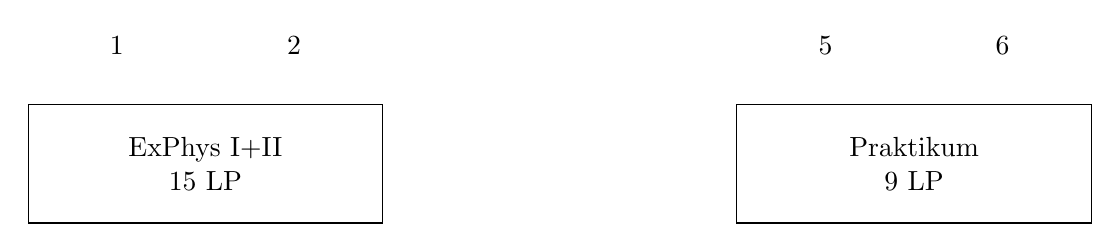
\begin{tikzpicture}
		\colnr{0}{1}{1}
		\colnr{1}{1}{2}
		\colnr{4}{1}{5}
		\colnr{5}{1}{6}
	    \doublemodul{0}{0}{ExPhys~I+II\\15 LP}
	    \doublemodul{4}{0}{Praktikum\\9 LP}
		
    \end{tikzpicture}
\end{center}
Am Ende des Moduls \glqq Grundlagen der Experimentalphysik I\grqq\ 
steht eine dreistündige Klausur.
Die Note aus dieser Klausur ist zugleich eure Nebenfachnote.
Außerdem braucht man den Schein aus dem \glqq Physikalischen Praktikum~I\grqq.

%%%%%%%%%%%%%%%%%%%%%%%%%%%%%%%%%%%%%%%%%%%%%%%%%%%%%%%%%
%% Stand: 31. August 2010
%%%%%%%%%%%%%%%%%%%%%%%%%%%%%%%%%%%%%%%%%%%%%%%%%%%%%%%%%


\subsubsection{Nebenfach Technische Mechanik} 

Technische Mechanik (TM) als Nebenfach bildet
eine Brücke zu den Ingenieurwissenschaften.

Mechanik unterteilt sich in die Kinematik,
die Lehre von den Bewegungen, 
und die Dynamik, die Lehre von Kräften.
Die "`technische"' Mechanik beschränkt sich
auf die Anwendungen in der Technik,
d.h.\ Biomechanik oder Himmelsmechanik
werden zum Beispiel nicht behandelt.

Natürlich ist die Mechanik ein Teilgebiet der Physik.
Dies bedeutet jedoch nicht,
dass man Vorkenntnisse aus der Physik mitbringen 
oder gar ein gro"ses Interesse an der Physik haben muss.

Die Vorlesungen geben einen schönen Einblick
in die Arbeitsweise der Ingenieure.
Hier werden "`real existierende"' Probleme analysiert
und in ein mathe\-mati\-sches Modell übertragen,
d.h.\ man versucht das Problem mit mathematischen Gleichungen
darzustellen und mit deren Hilfe zu lösen.
Damit ist auch schon gesagt,
dass die TM sehr viel mit Mathematik zu tun hat. 
Wer also nicht nur Mathematik abstrakt lernen,
sondern auch mal anwenden will,
für den ist TM als Nebenfach sehr zu empfehlen. 

Nebenbei sei noch erwähnt, dass die Mechanik-Institute
der Universität an Mathematikern interessiert sind.
Mathematik-Studierende sind dort zwar seltene,
aber gern gesehene Gäste.

\begin{center}
\begin{tabular}{|@{}c@{}|@{}c@{}|@{}c@{}@{}c@{}|@{}c@{}@{}c@{}} 
\multicolumn{1}{c}{\makebox[2.4cm]{1}}&\multicolumn{1}{c}{\makebox[2.4cm]{2}}&
\multicolumn{1}{c}{\makebox[2.4cm]{3}}&\multicolumn{1}{c}{\makebox[2.4cm]{4}}&
\multicolumn{1}{c}{\makebox[2.4cm]{}}&\multicolumn{1}{c}{\makebox[2.4cm]{}}\\[0.2cm] 
\cline{1-4}
\bf TM~I&\multicolumn{2}{c|}{\bf TM~II+III}&\bf TM~IV~M&&\\
\it6 LP&\multicolumn{2}{|c|}{\it12 LP}&\it6 LP&\\
\cline{1-4}
 \end{tabular}
\end{center}
Aus den Modulen \glqq Technische Mechanik I\grqq
~und \glqq Technische Mechanik II+III\grqq~benötigt man einen Schein,
das Modul \glqq Technische Mechanik IV
für Mathematiker\grqq~hat am Ende eine Prüfung.
Die Note dieser Prüfung ist die Nebenfachnote.
Bei allen Fragen zu TM ist Prof.~Peter Eberhard
(\texttt{eberhard@itm.uni-stuttgart.de}) gerne bereit, dir weiterzuhelfen.


%\vspace{3cm}
%\begin{center}
%\epsfig{file=hagar.ps,width=14cm}
%\end{center}


\subsubsection{Nebenfach Technische Biologie}
Technische Biologie ist eine außergewöhnliche Verbindung klassischer,
biochemischer und molekularbiologischer Inhalte mit modernen Techniken:
Im Fokus steht oft ein direkter Anwendungsbezug.
Dabei können Mathematik und Technische Biologie
in hohem Maße wechselseitig voneinander profitieren
und sogar völlig neue Forschungsansätze hervorbringen.
Die Mathematik bietet z.B.\ hervorragende Modelle,
um biologische Systeme besser zu verstehen,
während in der belebten Welt bestimmte mathematische Prinzipien
dominieren und dadurch Indizien für besonders
erfolgsversprechende Strategien liefern. 
Leider sind die Überschneidungen der Vorlesungen
nicht unerheblich - du brauchst also einiges an Ausdauer,
um dieses Nebenfach zu studieren.

\begin{center}
 \begin{tabular}{|@{}c@{}|@{}c@{}|@{}c@{}@{}|} 

   \multicolumn{1}{c}{\makebox[2.4cm]{1}} &
   \multicolumn{1}{c}{\makebox[2.4cm]{2}}  & \multicolumn{1}{c}{\makebox[2.4cm]{3}} \\[0.2cm] 

\cline{1-2} \cline{2-3}

  \multicolumn{1}{|c|}{\bf Techn.~Bio I für NF}       & \multicolumn{1}{c|}{\bf Techn.~Bio II für NF} & \multicolumn{1}{c|}{\bf Techn.~Bio III für NF}  \\
       \it 9 LP       & \it 6 LP &    \it 3 LP  \\

\cline{1-2} \cline{2-3}

 \multicolumn{1}{c}{} &  & \multicolumn{1}{c|}{\bf Bioinfo.~\& Biostat.}  \\
\multicolumn{1}{c}{} &  & \multicolumn{1}{c|}{\it 6 LP}  \\ \cline{3-3}

 \end{tabular}
\end{center}
Alle Module schließen mit einer Prüfung ab.
Die Nebenfachnote ist der Mittelwert aller Module.
Mit Ausnahme des Moduls \glqq Biophysikalische Chemie I\grqq
~benötigt man zudem zu jedem Modul einen Schein.

%%%%%%%%%%%%%%%%%%%%%%%%%%%%%%%%%%%%%%%%%%%
%% Stand: 31. August 2010
%%%%%%%%%%%%%%%%%%%%%%%%%%%%%%%%%%%%%%%%%%%


\subsubsection{Nebenfach Technische Kybernetik}

Kybernetik ist - als Teilgebiet der Systemwissenschaft
- die Lehre der Kommunikation und Regelung
von lebenden Organismen und Maschinen und
wird auch als die Kunst des Steuerns bezeichnet.
Die Kybernetik erforscht die grundlegenden Konzepte
zur Steuerung und Regulation von Systemen und
hat einen starken mathematischen Bezug.
Durch die interdisziplinäre Ausrichtung
bietet sich der Kybernetik ein vielfältig und
breitgefächertes Anwendungsspektrum,
das Absolventen hervorragende Berufsmöglichkeiten bietet.

\vspace*{-1cm}

\begin{center}
 \begin{tabular}{|@{}c@{}|@{}c@{}|@{}c@{}|@{}c@{}|@{}c@{}|@{}c@{}} 

   \multicolumn{1}{c}{\makebox[2.4cm]{1}} &
   \multicolumn{1}{c}{\makebox[2.4cm]{2}}  & \multicolumn{1}{c}{\makebox[2.4cm]{3}} &
   \multicolumn{1}{c}{\makebox[2.4cm]{4}} &
   \multicolumn{1}{c}{\makebox[2.4cm]{5}}  & \multicolumn{1}{c}{\makebox[2.4cm]{}} \\[0.2cm] 

\cline{1-5}

  \multicolumn{2}{|c|}{\bf ExPhys I+II}                &\bf Projekt &\bf S.dynamik&\bf Regelungst.&  \\
  \multicolumn{1}{|c}{3+2}& \multicolumn{1}{c|}{4+2}& \it 3 LP& \it 3 LP& \it 3 LP&  \\
\cline{3-5}
  \multicolumn{2}{|c|}{\it 15 LP}                   &\multicolumn{4}{c}{}  \\
 \cline{1-2}
 \end{tabular}
\end{center}
Von der \glqq Projektarbeit Technische Kybernetik\grqq~(meist Teilnahme am Roborace) benötigt man einen Schein, alle anderen Module schließen mit einer Prüfung ab. Es gilt:\\[0.5ex]
\begin{tabular}{lcrl}
Nebenfachnote & = &$\frac{15}{27}\,\cdot$ &Grundlagen der Experimentalphysik~I\\[0.5ex]
              & + &$\frac{6}{27}\,\cdot$ &Systemdynamik\\[0.5ex]
              & + &$\frac{6}{27}\,\cdot$ &Einführung in die Regelungstechnik\\ 
\end{tabular}

%%%%%%%%%%%%%%%%%%%%%%%%%%%%%%%%%%%%%%%%%%
%%  Stand: 31. August 2010
%%%%%%%%%%%%%%%%%%%%%%%%%%%%%%%%%%%%%%%%%%


\subsubsection{Nebenfach Luft- und Raumfahrttechnik}

Die Luft- und Raumfahrttechnik (LRT)
ist eine der Ingenieurwissenschaften,
für die die Universität Stuttgart bekannt ist.
Auch das Deutsche Zentrum für Luft- und Raumfahrt
ist am Campus vertreten und kooperiert fleißig mit der Uni.
LRT ist ein eher anspruchsvolles Nebenfach.

\vspace*{-1cm}

{\small\begin{center}\begin{tabular}{|@{}c@{}|@{}c@{}|@{}c@{}|@{}c@{}|@{}c@{}|@{}c@{}} 
\multicolumn{1}{c}{\makebox[2.4cm]{1}}&\multicolumn{1}{c}{\makebox[2.4cm]{2}}&
\multicolumn{1}{c}{\makebox[2.4cm]{3}}&\multicolumn{1}{c}{\makebox[2.4cm]{4}}&
\multicolumn{1}{c}{\makebox[2.4cm]{5}}&\multicolumn{1}{c}{\makebox[2.4cm]{6}}\\[0.2cm]
\hline
\multicolumn{2}{|c|}{\bf Physik+Elektronik}&\bf Thermodyn&
\bf Strömungsl&\multicolumn{2}{c|}{\bf Prak.~Strömungssim.}\\
\multicolumn{1}{|c}{   }&\multicolumn{1}{c|}{   }&
\multicolumn{2}{c|}{    \quad {\it oder} \quad    }&
\multicolumn{1}{c}{   }&\multicolumn{1}{c|}{    \it 3 LP}\\
\cline{6-6}
\multicolumn{2}{|c|}{\it6 LP}&\it6 LP&\it6 LP&
\multicolumn{1}{c|}{\it oder }&\\
\cline{1-4}
\bf TM~I&\bf TM~II&\multicolumn{2}{c|}{}&\bf Luftfahrt&\\
\multicolumn{1}{|c|}{}&&\multicolumn{2}{c|}{}&\it3 LP&\\
\it6 LP&\it6 LP&\multicolumn{2}{c|}{}&\it oder&\\
\cline{1-2}
\multicolumn{4}{c|}{}&\bf Strömung&\\
\multicolumn{4}{c|}{}&\it3 LP&\\
\cline{5-5}
\end{tabular}\end{center}}

Man wählt zwischen \glqq Grundlagen der Thermodynamik~I\grqq\ (drittes Semester)
und \glqq Strömungslehre~I\grqq\ (viertes Semester).

Außerdem hat man die Wahl zwischen
\glqq Rechnerpraktikum Strömungssimulation\grqq,
\glqq Einführung in die Luftfahrttechnik\grqq\ 
und \glqq Rechnerpraktikum Numerische Simulation
von Strömung und Wärmeleitung\grqq.

%\begin{tabular}{lcrl}
%Nebenfachnote & = &$\frac{2}{7}\,\cdot$&Physik und Elektronik für LRT\\[0.5ex]
%              & + &$\frac{2}{7}\,\cdot$&Technische Mechanik I\\[0.5ex]
%              & + &$\frac{1}{7}\,\cdot$&Technische Mechanik II\\[0.5ex]
%              & + &$\frac{2}{7}\,\cdot$&Grundl.\,der\,Thermodynamik\,I {\it oder} Strömungslehre\,I\\ 
%\end{tabular}

%%%%%%%%%%%%%%%%%%%%%%%%%%%%%%%%%%%%%%%%%%%%
%%  Stand: 31. August 2010
%%%%%%%%%%%%%%%%%%%%%%%%%%%%%%%%%%%%%%%%%%%%


\subsubsection{Philosophie}
Wir freuen uns, mit Philosophie auch ein nicht
naturwissenschaftliches Nebenfach anbieten zu können.
%{\small\begin{center}\begin{tabular}{|@{}c@{}|@{}c@{}|cc|@{}c@{}@{}|}
%\multicolumn{1}{c}{\makebox[2.4cm]{1}}&
%\multicolumn{1}{c}{\makebox[2.4cm]{2}}&
%\multicolumn{1}{c}{\makebox[1.6cm]{3}}&
%\multicolumn{1}{c}{\makebox[1.6cm]{4}}&
%\multicolumn{1}{c}{\makebox[2.4cm]{5}}\\[0.2cm]
%\cline{1-2}\cline{5-5}
%\multicolumn{1}{|c|}{\bf Grundl.~der Phil.}&
%\multicolumn{1}{c|}{\bf Einf.~in die prakt.~Phil.}&&&
%\multicolumn{1}{|c|}{\bf Theoretische Phil.}\\
%\it12 LP&\it6 LP&&&\it6 LP\\
%\cline{1-2}\cline{5-5}
%\end{tabular}\end{center}}

\begin{center}
	\begin{tikzpicture}
		\colnr{0}{1}{1}
		\colnr{1}{1}{2}
		\colnr{4}{1}{5}
	    \modul{0}{0}{GP\\12 LP}
	    \modul{1}{0}{EP\\6 LP}
		\modul{4}{0}{TP\\6 LP}
    \end{tikzpicture}
\end{center}
Mit GP bezeichnen wir die \glqq Grundlagen der Philosophie\grqq ,
mit EP die \glqq Einführung in die praktische Philosphie\grqq
und mit TP die \glqq theoretische Philosophie \grqq.

%%%%%%%%%%%%%%%%%%%%%%%%%%%%%%%%%%%%%%%%%%%%
%%  Stand: 31. August 2010
%%%%%%%%%%%%%%%%%%%%%%%%%%%%%%%%%%%%%%%%%%%%


\subsection{Schlüsselqualifikationen}

Von Bachelor-Studenten wird erwartet,
dass sie sogenannte `Schlüsselqualifikationen'
(besser bekannt unter dem Namen `Soft Skills')
im Umfang von 18 LP erwerben.

Ein paar dieser Punkte erwirbst du automatisch
durch das Computerpraktikum.
Dies ist nämlich genau genommen kein Mathematikmodul,
sondern seine 6 LP gehören den Soft Skills an.

Von den restlichen 12 LP müssen genau 6 LP
in einer fachaffinen Veranstaltung erworben werden.
Dies sind zum Beispiel:\\[6pt]
- {\bf `Präsentation und Vermittlung von Mathematik'} (3 LP)\\[2pt]
- {\bf `Computertutorium Mathematik'} (3 LP)\\[2pt]
- {\bf Nebenfach-Module} (3 - 6  LP)\\[6pt]
Genau 6 LP müssen aus sogenannten fachübergreifenden
Schlüsselqualifikationen stammen.
Ein entsprechender Katalog für diese uniweit angebotenen
Veranstaltungen wird rechtzeitig bekannt gegeben.
Die Anmeldung erfolgt auch hier über das C@mpus
in einem gewissen Zeitraum.

\vspace*{2cm}
\begin{center}
\includegraphics[width=\textwidth]
{/afs/.stud.mathe/fsmath/gemeinsame_Bilder/Comics/comic435}
\end{center}

%%%%%%%%%%%%%%%%%%%%%%%%%%%%%%%%%%%%%%%%%%%%%%%%%%%%
%% Stand: 31. August 2010
%%%%%%%%%%%%%%%%%%%%%%%%%%%%%%%%%%%%%%%%%%%%%%%%%%%%


\newpage
\section{Studienplan des Bachelor of Arts für's Lehramt}\label{LA}

Den Studienplan für dein Zweitfach hier aufzuführen,
würde den Rahmen dieses Infoheftes sprengen,
darum beschränken wir uns auf die
von dir verlangten Leistungsnachweise in Mathematik.
Falls du wichtige Fragen zum Lehramtsstudium haben solltest,
gehe bitte zum Lehramtszuständigen (siehe \ref{LAzust})
oder schau bei uns in der Fachgruppe vorbei.

\subsection{Der Mathematikanteil}
Zu Beginn des Studiums wirst du folgende Grundvorlesungen hören:\\[6pt]
- {\bf Analysis~I}\\[2pt]
- {\bf Analysis~II}\\[2pt]
- {\bf Lineare Algebra und Analytische Geometrie~I} (LAAG I)\\[2pt]
- {\bf Lineare Algebra und Analytische Geometrie~II} (LAAG II)\\[6pt]
Wenn für dich Mathematik die höhere Priorität hat,
kannst du diese Vorlesungen zum Beispiel
innerhalb der ersten zwei Semester absolvieren.
Dazu müsstest du LAAG und Analysis parallel hören.
Andernfalls könntest du zunächst LAAG~I+II in den ersten zwei Semestern
und im dritten und vierten Semester Analysis~I+II hören.
Natürlich könntest du auch mit Analysis beginnen,
dies können wir dir jedoch nicht empfehlen,
da du in Analysis II die Lineare Algebra benötigst. 
Zu jedem dieser Module musst du eine schriftliche Prüfung ablegen.
Prüfungsvorleistung ist immer der jeweilige Schein.
Deine Orientierungsprüfung besteht
entweder aus der Modulprüfung zu LAAG I oder aus der Modulprüfung zu Analysis I,
diese musst du bis zum Beginn der Vorlesungszeit
des vierten Semesters bestanden haben. 
Wenn du einen Großteil der oben genannten Module absolviert hast,
kannst du dich an folgende Module machen:\\[6pt]
- {\bf Algebra und Zahlentheorie für gym. Lehramt} {\em oder}\\[2pt]
   \quad  {\bf Analysis~III}\\[2pt]
- {\bf Mathematische Programmierung für gym. Lehramt}\\[2pt]
- {\bf Stochastik und Angewandte Mathematik für gym. Lehramt}\\[2pt]
- {\bf Geometrie für gym. Lehramt}\\[2pt]
- {\bf Komplexe Analysis für gym. Lehramt}\\[2pt]
- {\bf Fachdidaktik~I}\\[6pt]

Dir ist es erlaubt zwischen Analysis~III und Algebra und Zahlentheorie zu wählen.
\begin{center}
\includegraphics[width=17cm]
{/afs/.stud.mathe/fsmath/gemeinsame_Bilder/Friederike/Lehramt1}
1. Priorität Mathematik
\end{center}
Für das Erste ist es empfohlen Analysis~I+II gehört zu haben und
für das Zweite solltest du Ahnung von LAAG~I+II haben.
Du solltest nur bedenken, dass du das was du nicht wählst, im Master hören musst.
Das Modul mathematische Programmierung setzt sich aus einem
Programmierkurs und einer größeren Programmieraufgabe zusammen.
Anschließend erkundest du die Welt der Stochastik und angewandten Mathematik. 
Um dich an Geometrie heranzuwagen, solltest du alle Grundvorlesungen hinter dir haben.
An die komplexe Analysis darfst du bereits ran, wenn du Analysis~I+II gemeistert hast.
Wie die Prüfungen genau aussehen
und ob ein Schein Prüfungsvorleistung ist,
erfährst du vom jeweiligen Dozenten zu Beginn der Veranstaltung.
Außerdem brauchst du ein Proseminar im Umfang von 3 LP.
\begin{center}
\includegraphics[width=17cm]
{/afs/.stud.mathe/fsmath/gemeinsame_Bilder/Friederike/Lehramt2}
2. Priorität Zweitfach
\end{center}
Zum Abschluss deines Bachelor of Arts ist in einem deiner beiden Fächer
eine kurze wissenschaftliche Arbeit (Bachelorarbeit) zu schreiben.
Diese hat einen Umfang von 6 LP.
%Das Modul angewandte Mathematik setzt sich zusammen
%aus einer Vorlesung mit Übung zur \glqq Wahrscheinlichkeitstheorie\grqq\ 
%(Zulassungsvoraussetzung hierfür: Analysis~I+II),
%einem Programmierkurs und eine Vorlesung zur
%\glqq Numerischen Lineare Algebra\grqq\ mit Übung
%(empfohlene Voraussetzung hierfür: LAAG~I).
%Als inhaltliche Voraussetzung für die Einführung
%in die Geometrie und Algebra
%werden LAAG~I+II empfohlen.
\subsection{Spezielle Veranstaltungen fürs Lehramt}

\subsubsection{Bildungswissenschaften}

Für Lehrämtler im Bachelor of Arts
sind einige Pädagogikveranstaltungen Pflicht.
Während deinem Studium wirst du folgende Module besuchen:\\[6pt]
- {\bf Bildungswissenschaftliche Grundlagen I:}\\
\ \ Einführung in die pädagogische Psychologie (Vorlesung, 1.~Semester)\\[2pt]
- {\bf Bildungswissenschaftliche Grundlagen II:}\\
\ \ Erziehungswissenschaftliches Arbeiten (Seminar, 1.~oder 3.~Semester)\\[2pt]
- {\bf Schulpraktische Orientierung:}\\
\ \ Analyse von Lehr- und Lernprozessen I (Seminar, 2.~Semester)\\[2pt]
- {\bf Lehren und Lernen:}\\
\ \ Didaktik (Vorlesung, 3. oder 5.~Semester)\\[2pt]
- {\bf Schulpraktische Orientierung:}\\
\ \ Orientierungspraktikum (Praktikum, 3.~oder 4.~Semester)\\[2pt]
- {\bf Lehren und Lernen:}\\
\ \ Analyse von Lehr- und Lernprozessen II (Seminar, 4.~Semester)\\[2pt]
Die Semesterangaben sind Empfehlungen,
aber in keinster Weise prüfungsrechtlich bindend.
Du solltest aber die Voraussetzungen der Module beachten:
Es ist B.W.~Grundl.~I Voraussetzung für B.W.~Grundl.~II
und Analyse von Lernprozessen~I
Voraussetzung für Analyse von Lernprozessen~II.
Es wird empfohlen, das Orientierpraktikum frühzeitig abzulegen,
denn es soll dir eine Vorstellung davon geben,
wie dein Lehrerberuf in Zukunft aussieht.

%% Im Fall des Orientierungspraktikums
%% handelt es sich um eine indiskutable Frist,
%% die unter allen Umständen eingehalten werden muss,
%% ähnlich wie die Orientierungsprüfung.

{\it Weitere ausführliche Infos/Quelle:}\\
{\small\verb|http://www.uni-stuttgart.de/studieren/angebot/lehramt/la_bama/la_bama.pdf|}

\begin{center}
\includegraphics[width=17cm]
{/afs/.stud.mathe/fsmath/gemeinsame_Bilder/Comics/certainty}
\end{center}

\subsubsection{Orientierungspraktikum}

Im Verlauf deines Studiums im Bachelor of Arts
musst du ein Orientierungspraktikum absolvieren.
Du besuchst in dieser Zeit eine Schule (nicht deine eigene)
und kannst so einen Eindruck gewinnen,
ob dir der Lehrerberuf gefallen könnte.
Das Orientierungspraktikum liefert 3 LP.\\
Zum Orientierungspraktikum muss man sich anmelden.
Nähere Informationen findest du unter:
\verb|http://www.orientierungspraktikum-bw.de/|\\
Die eigentliche Schulpraxis kommt erst im anschließenden
Master of Education.
Da wirst du ein Schulpraxismodul
von einem Umfang von 16 LP absolvieren.

{\small P.S.: Aufgrund eines Übertragungsfehlers
kursiert die Information,
das Orientierungspraktikum müsste schon
bis zu Beginn des 4.\ Semesters absolviert sein.
Dies trifft nicht zu, es wird aber trotzdem empfohlen,
das Orientierungspraktikum zeitig zu absolvieren.}

\vspace*{1cm}

%% \subsubsection{Schulpraktikum}
%% Das Schulpraktikum ist ein eigenes Modul mit 16 LP.
%% Es findet in einem ungeraden Semester (vorgesehen ist das fünfte Semester,
%% also nach der Zwischenprüfung) statt und
%% geht über 13 Wochen ab Schulbeginn im September.
%% \linebreak In dieser Zeit besuchst Du eine Schule,
%% beobachtest den Unterricht von anderen Lehrern
%% (man sagt auch \glqq hospitieren\grqq) und darfst auch
%% selbst erste Unterrichtserfahrung sammeln. \\
%% Das Schulpraxissemester kann bestanden
%% oder auch nicht bestanden werden.
%% Wenn du das Praktikum nicht bestehst,
%% kannst du es einmal wiederholen.
%% Auch zum Schulpraktikum musst du dich anmelden:\\

%% %\vspace*{0.5 cm}
%% Der Anmeldezeitraum ist vom ersten Schultag
%% nach den Osterferien bis zum 15.05., mind. jedoch 4 Wochen,
%% und erfolgt in zwei Schritten:
%% \begin{center}
%% \begin{itemize}
%%   \item
%%     Seminarplatz für das Praxissemester an einer Schule im Internet reservieren. 
%%     Eine Reservierung an mehreren Schulen ist nicht gleichzeitig möglich.
%%   \item
%%     Irgendwann meldet sich dann die Schule. Meistens muss man noch zu einem
%%     persönlichen Gespräch dorthin, das aber nur dazu dient, sich schon mal
%%     kennenzulernen.
%% \end{itemize}
%% \end{center}
%% Unter \verb|http://www.praxissemester-bw.de/| oder
%% natürlich bei uns in der Fachgruppe findest du weitere Informationen.
%% Es gibt auch die Möglichkeit, das Orientierungs-
%% und Schulpraktikum im Ausland zu absolvieren.
%% Details findest du auch dazu im Internet.
%% Wichtig ist in diesem Fall, sich frühzeitig zu informieren.




%%%%%%%%%%%%%%%%%%%%%%%%%%%%%%%%%%%%%%%%%%
%% Stand: 03. Oktober 2016
%%%%%%%%%%%%%%%%%%%%%%%%%%%%%%%%%%%%%%%%%%


\newpage
\section{Die Fachgruppe Mathematik}

Was ist das: Fachgruppe\,?\\

In diesem Kapitel möchten wir dir erklären,
was die {\bf Fachgruppe} ist und was sie so alles macht.

Die Fachgruppe sieht sich als Interessenvertretung
aller Mathematik--Studenten und
betreibt ausschließlich \glqq Hochschulpolitik\grqq .
Wir sind also ganz normale Studenten,
die neben ihrem Studium noch Zeit investieren,
um für gute Studienbedingungen an unserer Universität zu sorgen.
%\vspace*{0.5cm}
\ifthenelse{\boolean{online}}
{
}
{
\begin{center}
\includegraphics[width=\textwidth]{afs/.stud.mathe/fsmath/gemeinsame_Bilder/Comics/shoe_algebra}
\end{center}
}

Neben dieser Interessenvertretung der Studenten
wollen wir auch eine allgemeine Studienberatung sein.
{\bf Wann immer irgendwelche Probleme oder Fragen
     bezüglich des Studiums auftauchen,
     kannst du dich jederzeit an uns wenden.} 
Wir haben in der Regel einen guten Kontakt zu den Professoren
und wissen meist auch Bescheid,
welche Person in unserer Fakultät für was zuständig ist.
Vielleicht können wir nicht jede deiner Fragen beantworten,
aber zumindest können wir dich an zuständige Personen verweisen.

Hier ist eine Auf\-listung der Dinge,
die wir die ganze Zeit so machen:

\begin{itemize}

% Erstsemester
\item
Dieses {\bf Erstsemesterinformationsheft} (ESI),
das du gerade liest, wurde zum Beispiel von der
Fachgruppe zusammengestellt und geschrieben. 
Ebenso organisieren wir vor jedem Wintersemester
die {\bf Erstsemestereinführung} (ESE), um denen,
die neu an die Uni kommen und sich überhaupt noch nicht auskennen,
ein wenig mit Rat und Tat zur Seite zu stehen.
Dieses Jahr findet diese Erstsemestereinführung
am \ESETagEins. und \ESETagZwei.~Oktober statt. 
 
%Tage
\item
Die Fachgruppe beteiligt sich an vielen {\bf Informationsveranstaltungen}
(Tag der Wissenschaft, Unitag ,\dots).
Dort machen wir Werbung für das Mathematikstudium
und geben wichtige Hinweise an Schüler,
was sie alles in der Mathematik erwarten wird.
Vielleicht hast du uns ja schon einmal auf einer dieser Veranstaltungen gesehen.

%Vorlesungsumfrage
\item
Die {\bf Vorlesungsumfrage} wird von uns ausgewertet
und ist eine Möglichkeit, den Professoren
eine Rückmeldung zur ihrer Vorlesung zu geben.

%Seminarplatzvergabe
\item
Die Fachgruppe sorgt jedes Semester dafür,
dass es eine {\bf Pro- und Hauptseminarplatzvergabe}
(meistens am letzten Mittwoch in der Vorlesungszeit) gibt.
Dort werden die freien Plätze für die Seminare
des darauffolgenden Semesters vergeben.
\end{itemize}

\ifthenelse{\boolean{online}}
{
}
{
\begin{center}
\includegraphics[width=16cm]
{afs/.stud.mathe/fsmath/gemeinsame_Bilder/Comics/mathreli}
\end{center}
}

\begin{itemize}
%ROMCE
\item
Au"serdem veranstaltet die Fachgruppe für alle Mathematiker
im Sommer- und im Wintersemester das ROMCE, unser {\bf Spielewochenende},
wo wir gemeinsam ein (verlängertes) Wochenende in einer Jugendherberge verbringen.
Dieses Wochenende ist insbesondere für Erstsemester
gedacht und soll Gelegenheit bieten, sich untereinander kennenzulernen,
denn gemeinsam geht vieles besser
(siehe letzten Abschnitt).

%Prüfungsprotokolle
\item
Damit die Vorbereitung auf Prüfungen besser läuft,
haben wir für euch diverse {\bf Prüfungsprotokolle} von vergangenen Prüfungen.
Schriftliche Prüfungen aus den letzten Jahren
findet ihr auf unserer Internetseite (nur vom Uni-Netz aus zugänglich),
Protokolle von mündlichen Prüfungen gibt es in der Fachgruppe gegen Pfand.

\item
Die Fachgruppe verkauft  {\bf Getränke} und {\bf Sü"sigkeiten}
zum Selbstkostenpreis, damit von unseren Studenten
auch keiner verdursten muss und jeder etwas Nervennahrung für die Vorlesungen hat.

\item
Weiterhin bietet die Fachgruppe auch eine relativ große Sammlung an Spielen an.
Die Spiel könnt ihr gerne, nach Feststellung eurer Personalien, für kurze Zeit ausleihen.
\end{itemize}

Neben den direkt sichtbaren Serviceleistungen gibt es
auch noch jede Menge von laufenden Aufgaben,
von denen viele Studenten kaum etwas merken,
die aber trotzdem wichtig sind. Dazu zählen unter anderem:

\begin{itemize}
\item
Die {\bf Fachgruppensitzung}:
Die Fachgruppe trifft sich in der Vorlesungszeit
einmal pro Woche zur Fachgruppensitzung,
zu der alle Studenten recht herzlich eingeladen sind.
In der Fachgruppensitzung wird alles besprochen,
was gerade so anliegt, z.B.\ Beteiligung an Uni-Veranstaltungen,
Organisation von Fachgruppen-Angeboten (s.o.),
Änderungen an Studienbedingungen und vieles mehr.\\
{\bf Nächster Termin:} Wird stets auf unserer Homepage angekündigt.

\item
{\bf Fachbereichs-/Fakultätsratsvertreter}:
Die Fachgruppe hat voll stimmberechtigte studentische Vertreter
im Fachbereichsrat (Mathematik) und Fakultätsrat (Mathematik/Physik),
den beiden zentralen Gremien für alle Belange des Mathematikstudiums.

\item
Die {\bf Studienkommission}:
Sie kümmert sich um die Studienordnung.
Insbesondere bei der Anpassung von Prüfungsordnungen,
aber auch bei der Verwendung von Studiengebühren
spielt sie eine wichtige Rolle.
Wir sind in diesem Gremium mit vier Leuten vertreten.

\item
Die {\bf Berufungskommissionen}:
Auch wenn es darum geht, neue Professoren auszusuchen
(um ausscheidende Professoren zu ersetzen)
haben die Studenten ein Mitspracherecht.
Wir achten darauf, dass bei den Auswahlkriterien
die Lehre nicht allzu kurz kommt
(die Professoren berücksichtigen in erster Linie die
Forschungsleistung und nicht die Qualität der Lehre).

\item
Der {\bf Fachschaftsrat} und die {\bf Stuvus}:
Die Fachgruppe entsendet Vertreter zum Fachschaftsrat,
der Interessenvertretung der Studenten der Fakultät $8$
(Mathematik und Physik).
Der Vorsitzende besitzt Stimmrecht im Studierendenparlament
der Studierendenvertretung Universität Stuttgart, kurz Stuvus. 

\newpage
Das Studierendenparlament ist das Legislativ-Organ
der Studierendenschaft der Uni Stuttgart.
Hier wird z.B.\ über Satzungen und Haushaltspläne abgestimmt,
d.\,h. unter anderem wie euer Studierendenschaftsbeitrag
von $5$\euro\ verwendet wird.
Ausserdem sind dort die uniweiten Arbeitskreise angesiedelt
z.B.\ AK Cräsh (Musikanlage), AK~Computer, AK~Umsetzbar, \dots \\
\end{itemize}

So, nun hast du einen groben Überblick darüber,
wer wir sind und was wir machen.
Wenn du Lust und Zeit hast, dann schau einfach mal vorbei,
wir freuen uns über jedes neue Gesicht. \\

Au"serdem:
Fachgruppe macht Spaß! Woran man das sieht?
- Na, warum sind wir sonst hier.

\begin{flushright}{\it Die Fachgruppe}\end{flushright}

\vspace*{3cm}
\ifthenelse{\boolean{online}}
{

}
{
\begin{center}
\includegraphics[width=8cm]
{afs/.stud.mathe/fsmath/gemeinsame_Bilder/Comics/snoopy}
\end{center}
}

%%%%%%%%%%%%%%%%%%%%%%%%%%%%%%%%%%%%%%%%
%%% Stand: 1. Juli 2010
%%%%%%%%%%%%%%%%%%%%%%%%%%%%%%%%%%%%%%%%


\newpage
\section{Was sonst noch interessiert...}

\subsection{Anlaufstelle für Mathestudenten}

Neben der Fachgruppe als Ansprechpartner,
könnt ihr euch auch jederzeit an {\bf Dr.~Friederike Stoll}
(Zimmer 7.553, Tel.: 0711/ 685-65515,
E-Mail: {\tt stoll@mathematik.uni-stuttgart.de}) wenden.
Sie kann euch bei organisatorischen Problemen jeglicher Art weiterhelfen.


\subsection{Ausbildungsförderung: BAföG}

Studieren kostet Geld: Miete, Essen, Trinken, Fahrkarten und Bücher --
auch wenn ihr zu Hause wohnt.
Nach Berechnungen des Studentenwerkes sind dies über 500\euro\ im Monat.
Dafür müssen i.d.R.\ eure Eltern aufkommen.
Verdienen sie aber nicht genug,
so habt Ihr Anspruch auf Berufsausbildungsförderung
nach dem Berufsausbildungsförderungsgesetz, kurz BAföG.

{\large \bf Wo und wie beantragt man BAföG?}

BAföG beantragt man beim

\begin{center}\begin{tabular}{|ll|}\hline
\multicolumn{2}{|l|}{Studierendenwerk Stuttgart}\\
\multicolumn{2}{|l|}{Amt für Ausbildungsförderung}\\
Holzgartenstrasse 11   & \\
70174 Stuttgart  & \\
\multicolumn{2}{|l|}{Tel. 0711 9574-509}\\\hline
\end{tabular}\end{center}

Antragsformulare gibt online unter\\
 \verb|https://www.studierendenwerk-stuttgart.de/antragsformulare| 

{\bf Wichtig:}
Gibt man den Antrag erst im November ab,
so verfällt das BAföG für Oktober.
Ist man knapp dran, so kann man den Antrag auch direkt
beim Amt für Ausbildungsförderung in den Briefkasten werfen.
Zur Fristwahrung reicht es, das Formblatt~1 --
das ist der eigentliche Antrag -- abzugeben,
die restlichen Unterlagen kann man nachreichen.


\newpage
{\large \bf BAföG-Beratung}

Informationen zum BAföG findet man beim Vaihinger Büro der FaVeVe
\glqq Hellblaues Nilpferd\grqq~(Tel.: 685-62004)
oder beim oben angegebenen Amt für Ausbildungsförderung.

%\begin{center}\begin{tabular}{|l|l|}\hline
%Beratungsstellen                  & Beratungszeiten            \\\hline\hline
%Amt für Ausbildungsförderung    & Mo. und Do. 9--11.30 Uhr  \\\hline
%Vaihinger Fachschaftenbüro       & Mo. 10--13 Uhr             \\
%~~\glqq Hellblaues Nilpferd \grqq & oder nach Vereinbarung     \\
%                                  & (Tel.: 685-62004)           \\\hline
%%\parbox[t]{4.5cm}{Vaihinger Fachschaftenbüro \glqq Hellblaues
%%  Nilpferd\grqq}  &\parbox[t]{6cm}{ Mo. 10--13 Uhr \par oder nach Vereinbarung (Tel.: %685-2004)} \\\hline
%\end{tabular}\end{center}

\begin{center}
\includegraphics[height=21cm]
{/afs/.stud.mathe/fsmath/gemeinsame_Bilder/Comics/substitute}
\end{center}


%%%%%%%%%%%%%%%%%%%%%%%%%%%%%%%%%
%%  Stand: 31. August 2010
%%%%%%%%%%%%%%%%%%%%%%%%%%%%%%%%%


\subsection{Gleichstellung}

Wie auch in einigen anderen Fachbereichen
ist der Frauenanteil in der Fakultät Mathematik
leider immer noch gering:
bei den Studierenden sind zwar ca. $50\,\%$  weiblich,
doch dieser Anteil wird immer niedriger,
je höher es in der Hierarchie geht.
Mit dieser Problematik beschäftigt sich -- fächerübergreifend --
die Gleichstellungsbeauftragte der Universität Stuttgart:
sie setzt sich dafür ein, dass gezielt Maßnahmen unternommen werden,
um die Studien-- und Arbeitssituation für Frauen an der
Universität zu verbessern und so den Frauenanteil allmählich zu erhöhen.
Dafür hat sie in jeder Fakultät eine/n Ansprechpartner/in
(meist eine Assistentin/wissenschaftliche Mitarbeiterin),
die speziell die Studentinnen und Mitarbeiterinnen
des jeweiligen Fachbereiches informiert und berät.
In der Fakultät Mathematik und Physik ist dies zur Zeit\\[2ex]
\hspace*{4cm} Dr.-Ing. Helga Kumric\\
\hspace*{4cm} Zimmer 3.159 \\
\hspace*{4cm} Tel. 0711/ 685-62197 \\
\hspace*{4cm} E-Mail h.kumric@physik.uni-stuttgart.de\\[2ex]
Bei Fragen, Problemen, Anregungen etc.\ 
zu diesem Bereich ist das also eine Anlaufstelle. 

\vspace{1cm}
\begin{center}
\includegraphics[width=\textwidth]
{afs/.stud.mathe/fsmath/gemeinsame_Bilder/Comics/dating_pools}
\end{center}

%%%%%%%%%%%%%%%%%%%%%%%%%%%%%%%%%%%%%%%%%%%%%
%%% Stand: 01. Juli 2010
%%%%%%%%%%%%%%%%%%%%%%%%%%%%%%%%%%%%%%%%%%%%%


\subsection{Nahverkehr}

{\large \bf Der "`VVS"' -- DAS NETZ}

(Fast) alle Busse und Bahnen des öffentlichen Personennahverkehrs
in Stuttgart und den vier umgebenden Landkreisen
gehören zum "`VVS"', dem Verkehrs- und Tarifverbund Stuttgart.

{\large \bf Mit dem Studentenausweis ab 18 Uhr durchs ganze Netz}

Vielleicht hast du dich schon gewundert,
dass du bei deiner (An- bzw.) Rückmeldung 166,50\euro\ überweisen musstest.
Von diesem Betrag gehen 44,50\euro\ an die VVS.
Dafür gilt dein gültiger Studentenausweis
(mit entsprechendem VVS-Aufdruck) täglich ab 18.00~Uhr
sowie an Wochenenden ganztags im ganzen Netz
das ganze Semester als Fahrausweis.
(Wintersemester: 1.~Okt.~- 31.~März, Sommersemster: 1.~Apr.~-30.~Sept.)
Diesen Beitrag musst du leisten,
ob du willst oder nicht bzw.~den VVS nutzt oder nicht.

{\large \bf Semesterticket (den ganzen Tag durchs ganze Netz)}

Wenn du täglich mit dem VVS zur Uni kommst,
was wahrscheinlich vor 18.00~Uhr geschieht,
gibt es eine zweite Komponente, das sogenannte "`Studiticket"'.
Hierfür musst du weitere 199,00\euro\ zahlen
und kannst dann das ganze Netz den ganzen Tag nutzen,
natürlich auch wieder das ganze Semster lang.
Dieses Ticket bekommt du bei allen SSB-Verkaufsstellen
und allen DB-Fahrkartenausgaben im VVS. 

{\large \bf Schwerbehinderte im Netz}

Studierende, die aufgrund einer Schwerbehinderung
zur kostenlosen Nutzung des Personennahverkehrs berechtigt sind,
erhalten auf Nachweis den Sockelbetrag von ca.\ 30\euro\ erstattet.

{\large \bf Verkaufsstellen und Kundenberatung}

Verkaufsstellen gibt es u.a.\ 
an der Universität direkt oben am S-Bahn-Ausgang
(der Haltestelle \glqq Universität\grqq, im runden Häuschen),
in der Klett-Passage und im Hauptbahnhof.
Für das obengenannte Semesterticket braucht du einen "`Verbundpass"',
für den du wiederum ein Lichtbild und eine
Immatrikulationsbescheinigung benötigst.\\
Seit 2013 kannst du das Ticket auch online kaufen,
was einige Vorteile bietet,
z.B.\ kannst du es bei Verlust einfach neu ausdrucken.\\[1cm]

%\newpage

{\it Mehr Infos bei}:\\
\\
\begin{tabular}{|l|l|l|}
\hline
VVS-Infothek & Kundenzentrum & Verkaufsstelle \\
Königsstr. 1A & Rotebühlpassage & Klettpassage (Hbf)  \\
Mo-Fr  9:00-18:30 Uhr & Mo-Fr 07:00-18:30 Uhr & Mo-Fr 07:00-19:45 Uhr \\
Sa 10:00-16:00 Uhr & & \\
\hline
\end{tabular}\\
\\
im Internet unter: \verb|http://www.vvs.de|

\newpage
\vspace*{5cm}
\begin{center}
\includegraphics[width=11cm]{afs/.stud.mathe/fsmath/gemeinsame_Bilder/Comics/comic10}
\end{center}

%%%%%%%%%%%%%%%%%%%%%%%%%%%%%%%%%%%%
%%% Stand: 23. 06. 2010
%%%%%%%%%%%%%%%%%%%%%%%%%%%%%%%%%%%%


\newpage
\subsection{Auslandsstudium}
 
Es mag manchem vielleicht etwas verfrüht erscheinen,
aber es gibt doch einige gute Gründe sich
über ein Auslandssemester oder -jahr zu informieren,
noch bevor das Studium an der Universität Stuttgart überhaupt begonnen hat.

Zum einen muss man mit den Vorbereitungen
bis zu anderthalb Jahren vor dem Auslandssemester beginnen.
Also im zweiten Semester, falls man im fünften Semester weg will,
was vermutlich die günstigste Zeit im Rahmen des Bachelors ist.

Vor allem aber wollen wir hier Werbung machen,
diese einmalige Chance zu nutzen.
Nicht nur, dass man natürlich seine Sprachfertigkeiten verbessert,
sondern vor allem die Erfahrung einer anderen Kultur,
der Beginn neuer Freundschaften -- in aller Welt --
und die Begegnung mit einer völlig anders gearteten Universitätskultur
-- die Mathematik bleibt allerdings dieselbe --
machen dies zu einem unvergesslichen Erlebnis.
All dies bleibt denen verborgen,
die solch einen Schritt nicht wagen.

Wer mehr über ein Auslandsstudium und die Möglichkeiten
dafür an der Uni Stuttgart wissen möchte,
sollte sich beim Amt für Internationale Angelegenheiten
(Pfaffenwaldring 60) erkundigen.
Die Uni hat  zahlreiche Kontakte zu ausländischen Hochschulen.
 %%% {}\hfill{\em Bernd Ackermann} 

\vspace{1cm}

\ifthenelse{\boolean{online}}
{

}
{
\vspace{1cm}
\begin{center}
\includegraphics[width=\textwidth]
{afs/.stud.mathe/fsmath/gemeinsame_Bilder/Comics/comic5}
\end{center}
}

%%%%%%%%%%%%%%%%%%%%%%%%%%%%%%%%%%%%%%%%
%%% Stand: 30.Juni 2010
%%%%%%%%%%%%%%%%%%%%%%%%%%%%%%%%%%%%%%%%


\newpage
\section*{Danksagung}

Wir bedanken uns bei unserer kompetenten
und stets hilfsbereiten Studiengangmanagerin Frau Dr.~Friederike Stoll,
die uns mit Rat und Tat bei der Erstellung
des Erstsemesterinfoheftes unterstützt hat.

\section*{Notizen~I}

Hier haben wir für dich noch ein bisschen Platz gelassen,
falls du dir ein paar Notizen direkt ins Heft machen möchtest.

\newpage
\section*{Notizen~II}


\newpage


\includepdf[pages=-]{stundenplan/stundenplan16_17.pdf}

\newpage
\subsection{Erstsemesterwochenende-ROMCE}
Du wirst es kaum glauben, aber unser ROMCE scheint tats"achlich die "alteste
Einrichtung des Fachbereichs Mathematik zu sein. Fragt man selbst
emeritierte Professoren (das sind Professoren im Ruhestand), so sagen diese,
dass es das eigentlich schon immer gab.

Dieses Semester werden wir mit dir in das Freizeitheim Geiststeinhöfle
in Walkersbach gehen.
Für Essen und Trinken sorgen wir alle gemeinsam
und werden uns so gut kennenlernen.
Insbesondere ist dies die Gelegenheit, die alten Hasen in geselliger Runde auszuquetschen.

Damit es uns abends nicht langweilig wird, werden wir auch noch eine Ladung Spiele
aus der Fachgruppe mitnehmen
und damit ein paar schöne Stunden verbringen.
%Falls dazu die Lust verloren geht, lassen wir uns irgendetwas Verrücktes einfallen.

Natürlich werden wir dort auch ein wenig (manche doch etwas mehr) Alkohol trinken.
Solange wir uns nicht wie die größten Deppen benehmen, sollte dies auch kein Problem sein.
\includepdf[pages=-]{plakat_16_17.pdf} 
%\vspace*{1cm}
%\begin{center}
%\includegraphics[width=1\linewidth, clip]
%{afs/.stud.mathe/fsmath/ROMCE/werbung/werbungWS1516/romce_werbung_esi_WS1516}
%\end{center}

%
%\centerline{\Huge \bf Spielewochenende \glqq ROMCE\grqq}
%\vspace{0.5cm}
%\centerline{\bf in der Jugendherberge in Creglingen}
%\vspace{0.5cm}
%\centerline{\Huge \bf \ROMCEAnfang. bis \ROMCEEnde. \ROMCEMonat {} \Jahreszahl}
%\vspace{1cm}
%Du wirst es kaum glauben, aber dies scheint tats"achlich die "alteste
%Einrichtung des Fachbereichs Mathematik zu sein. Fragt man selbst
%emeritierte Professoren (das sind Professoren im Ruhestand), so sagen diese,
%dass es das eigentlich schon immer gab. 
%
%Zweimal im Jahr st"urmen Horden von "uber und
%"uber mit Spielen beladenen Mathematikstudierenden die
%Jugendherberge in Creglingen.
%
%Neben Mathematikstudierenden aller Semester sind auch Ehemalige und
%Assistenten mit dabei. Selbstverst"andlich kannst du auch
%deine Freundinnen und Freunde, Ehepartner, Kinder und Geschwister
%mitbringen.
%
%Zus"atzlich zu Brett- und Gesellschaftsspielen kann man sich auch sportlich
%austoben. So geh"ort im Sommer das Beachvolleyballspiel ebenso zum Programm wie
%Spazierengehen, Inlineskaten, Tischfu"sball, Tischtennis, ...
%
%Bei viereinhalb Mahlzeiten am Tag kommen auch die k"orperlichen
%Gen"usse nicht zu kurz.
%
%Dieses Wochenende ist {\em die} M"oglichkeit, Kontakte zu Kommilitonen
%und H"ohersemestrigen herzustellen. 
%
%Nat"urlich wohnen wir nicht kostenlos in der Jugendherberge. Das komplette
%Wochenende kostet ca. 80\euro\ zuz"uglich Getr"anke.
%Anmelden kannst du dich im Fachgruppenzimmer.
%Mathematik. N"ahere Informationen werden rechtzeitig ausgeh"angt.
%
%Also sehen wir uns sp"atestens in der Jugendherberge in Creglingen!
%Bis dann!

%%%%%%%%%%%%%%%%%%%%%%%%%%%%%%%%%%%%%%%%%%%%%%%%%%%
%% Stand: 31. August 2010
%%%%%%%%%%%%%%%%%%%%%%%%%%%%%%%%%%%%%%%%%%%%%%%%%%%


\end{document}
